\documentclass[a4paper]{article}

\def\nterm {Fall}
\def\nyear {2018}
\def\nlecturer {Dr. Barry Ritchie}
\def\ncourse {Classical Particles, Fields, and Matter I}

\RequirePackage{etex}
\makeatletter
\ifx \nauthor\undefined
  \def\nauthor{Daniel Moore}
\else
\fi

\author{Based on lectures by \nlecturer \\\small Notes taken by \nauthor}
\date{\nterm\ \nyear}

\usepackage{alltt}
\usepackage{amsfonts}
\usepackage{amsmath}
\usepackage{amssymb}
\usepackage{amsthm}
\usepackage{booktabs}
\usepackage[makeroom]{cancel}
\usepackage{caption}
\usepackage{enumitem}
\usepackage{fancyhdr}
\usepackage{graphicx}
\usepackage{mathdots}
\usepackage{mathtools}
\usepackage{microtype}
\usepackage{multirow}
\usepackage{pdflscape}
\usepackage{pgfplots}
\usepackage{siunitx}
\usepackage{textcomp}
\usepackage{slashed}
\usepackage{tabularx}
\usepackage{tikz}
\usepackage{tikz-3dplot}
\usepackage{tkz-euclide}
\usepackage{titlesec}
\usepackage[normalem]{ulem}
\usepackage[all]{xy}
\usepackage{imakeidx}

\makeindex[intoc, title=Index]
\indexsetup{othercode={\lhead{\emph{Index}}}}
%\setcounter{secnumdepth}{4}

\titleformat{\paragraph}
{\normalfont\normalsize\bfseries}{\theparagraph}{1em}{}
\titlespacing*{\paragraph}
{0pt}{3.25ex plus 1ex minus .2ex}{1.5ex plus .2ex}

\ifx \nextra \undefined
  \usepackage[pdftex,
    hidelinks,
    pdfauthor={Daniel Moore},
    pdfsubject={\ncourse},
    pdftitle={\ncourse},
  pdfkeywords={\nterm\ \nyear\ \ncourse}]{hyperref}
  \title{\ncourse}
\else
  \usepackage[pdftex,
    hidelinks,
    pdfauthor={Daniel Moore},
    pdfsubject={\ncourse\ (\nextra)},
    pdftitle={\ncourse\ (\nextra)},
  pdfkeywords={\nterm\ \nyear\ \ncourse\ \nextra}]{hyperref}

  \title{\ncourse \\ {\Large \nextra}}
  \renewcommand\printindex{}
\fi

\pgfplotsset{compat=1.12}

\pagestyle{fancyplain}
\ifx \ncoursehead \undefined
\def\ncoursehead{\ncourse}
\fi

\lhead{\emph{\nouppercase{\leftmark}}}
\ifx \nextra \undefined
  \rhead{
    \ifnum\thepage=1
    \else
      \ncoursehead
    \fi}
\else
  \rhead{
    \ifnum\thepage=1
    \else
      \ncoursehead \ (\nextra)
    \fi}
\fi
\usetikzlibrary{arrows.meta}
\usetikzlibrary{decorations.markings}
\usetikzlibrary{decorations.pathmorphing}
\usetikzlibrary{positioning}
\usetikzlibrary{fadings}
\usetikzlibrary{intersections}
\usetikzlibrary{cd}

\newcommand*{\Cdot}{{\raisebox{-0.25ex}{\scalebox{1.5}{$\cdot$}}}}
\newcommand {\pd}[2][ ]{
  \ifx #1 { }
    \frac{\partial}{\partial #2}
  \else
    \frac{\partial^{#1}}{\partial #2^{#1}}
  \fi
}
\newcommand{\pder}[2]{
    \frac{\partial #1}{\partial #2}
}
\newcommand{\dd}[1]{
	\frac{\d}{\d #1}
}
\newcommand{\der}[2]{
	\frac{\d #1}{\d #2}
}
\newcommand{\mbeq}{\overset{!}{=}}
\newcommand{\vhat}[1]{\vec{\hat{#1}}}
\newcommand{\x}{\vhat{x}}
\newcommand{\y}{\vhat{y}}
\newcommand{\z}{\vhat{z}}
\newcommand{\del}{\vec{\nabla}}
\ifx \nhtml \undefined
\else
  \renewcommand\printindex{}
  \DisableLigatures[f]{family = *}
  \let\Contentsline\contentsline
  \renewcommand\contentsline[3]{\Contentsline{#1}{#2}{}}
  \renewcommand{\@dotsep}{10000}
  \newlength\currentparindent
  \setlength\currentparindent\parindent

  \newcommand\@minipagerestore{\setlength{\parindent}{\currentparindent}}
  \usepackage[active,tightpage,pdftex]{preview}
  \renewcommand{\PreviewBorder}{0.1cm}

  \newenvironment{stretchpage}%
  {\begin{preview}\begin{minipage}{\hsize}}%
    {\end{minipage}\end{preview}}
  \AtBeginDocument{\begin{stretchpage}}
  \AtEndDocument{\end{stretchpage}}

  \newcommand{\@@newpage}{\end{stretchpage}\begin{stretchpage}}

  \let\@real@section\section
  \renewcommand{\section}{\@@newpage\@real@section}
  \let\@real@subsection\subsection
  \renewcommand{\subsection}{\@ifstar{\@real@subsection*}{\@@newpage\@real@subsection}}
\fi
\ifx \ntrim \undefined
\else
  \usepackage{geometry}
  \geometry{
    papersize={379pt, 699pt},
    textwidth=345pt,
    textheight=596pt,
    left=17pt,
    top=54pt,
    right=17pt
  }
\fi

\ifx \nisofficial \undefined
\let\@real@maketitle\maketitle
\renewcommand{\maketitle}{\@real@maketitle\begin{center}\begin{minipage}[c]{0.9\textwidth}\centering\footnotesize These notes are not endorsed by the lecturers, and I have modified them (often significantly) after lectures. They are nowhere near accurate representations of what was actually lectured, and in particular, all errors are almost surely mine.\end{minipage}\end{center}}
\else
\fi

% Theorems
\theoremstyle{definition}
\newtheorem*{aim}{Aim}
\newtheorem*{axiom}{Axiom}
\newtheorem*{claim}{Claim}
\newtheorem*{cor}{Corollary}
\newtheorem*{conjecture}{Conjecture}
\newtheorem*{defi}{Definition}
\newtheorem*{eg}{Example}
\newtheorem*{ex}{Exercise}
\newtheorem*{fact}{Fact}
\newtheorem*{law}{Law}
\newtheorem*{lemma}{Lemma}
\newtheorem*{notation}{Notation}
\newtheorem*{prop}{Proposition}
\newtheorem*{question}{Question}
\newtheorem*{problem}{Problem}
\newtheorem*{rrule}{Rule}
\newtheorem*{thm}{Theorem}
\newtheorem*{assumption}{Assumption}

\newtheorem*{remark}{Remark}
\newtheorem*{warning}{Warning}
\newtheorem*{exercise}{Exercise}

\newtheorem{nthm}{Theorem}[section]
\newtheorem{nlemma}[nthm]{Lemma}
\newtheorem{nprop}[nthm]{Proposition}
\newtheorem{ncor}[nthm]{Corollary}


\renewcommand{\labelitemi}{--}
\renewcommand{\labelitemii}{$\circ$}
\renewcommand{\labelenumi}{(\roman{*})}

\let\stdsection\section
\renewcommand\section{\newpage\stdsection}

% Strike through
\def\st{\bgroup \ULdepth=-.55ex \ULset}


%%%%%%%%%%%%%%%%%%%%%%%%%
%%%%% Maths Symbols %%%%%
%%%%%%%%%%%%%%%%%%%%%%%%%

% Matrix groups
\newcommand{\GL}{\mathrm{GL}}
\newcommand{\Or}{\mathrm{O}}
\newcommand{\PGL}{\mathrm{PGL}}
\newcommand{\PSL}{\mathrm{PSL}}
\newcommand{\PSO}{\mathrm{PSO}}
\newcommand{\PSU}{\mathrm{PSU}}
\newcommand{\SL}{\mathrm{SL}}
\newcommand{\SO}{\mathrm{SO}}
\newcommand{\Spin}{\mathrm{Spin}}
\newcommand{\Sp}{\mathrm{Sp}}
\newcommand{\SU}{\mathrm{SU}}
\newcommand{\U}{\mathrm{U}}
\newcommand{\Mat}{\mathrm{Mat}}

% Matrix algebras
\newcommand{\gl}{\mathfrak{gl}}
\newcommand{\ort}{\mathfrak{o}}
\newcommand{\so}{\mathfrak{so}}
\newcommand{\su}{\mathfrak{su}}
\newcommand{\uu}{\mathfrak{u}}
\renewcommand{\sl}{\mathfrak{sl}}

% Special sets
\newcommand{\C}{\mathbb{C}}
\newcommand{\CP}{\mathbb{CP}}
\newcommand{\GG}{\mathbb{G}}
\newcommand{\N}{\mathbb{N}}
\newcommand{\Q}{\mathbb{Q}}
\newcommand{\R}{\mathbb{R}}
\newcommand{\RP}{\mathbb{RP}}
\newcommand{\T}{\mathbb{T}}
\newcommand{\Z}{\mathbb{Z}}
\renewcommand{\H}{\mathbb{H}}

% Brackets
\newcommand{\abs}[1]{\left\lvert #1\right\rvert}
\newcommand{\bket}[1]{\left\lvert #1\right\rangle}
\newcommand{\brak}[1]{\left\langle #1 \right\rvert}
\newcommand{\braket}[2]{\left\langle #1\middle\vert #2 \right\rangle}
\newcommand{\bra}{\langle}
\newcommand{\ket}{\rangle}
\newcommand{\norm}[1]{\left\lVert #1\right\rVert}
\newcommand{\normalorder}[1]{\mathop{:}\nolimits\!#1\!\mathop{:}\nolimits}
\newcommand{\tv}[1]{|#1|}
\renewcommand{\vec}[1]{\boldsymbol{\mathbf{#1}}}

% not-math
\newcommand{\bolds}[1]{{\bfseries #1}}
\newcommand{\cat}[1]{\mathsf{#1}}
\newcommand{\ph}{\,\cdot\,}
\newcommand{\term}[1]{\emph{#1}\index{#1}}
\newcommand{\phantomeq}{\hphantom{{}={}}}
% Probability
\DeclareMathOperator{\Bernoulli}{Bernoulli}
\DeclareMathOperator{\betaD}{beta}
\DeclareMathOperator{\bias}{bias}
\DeclareMathOperator{\binomial}{binomial}
\DeclareMathOperator{\corr}{corr}
\DeclareMathOperator{\cov}{cov}
\DeclareMathOperator{\gammaD}{gamma}
\DeclareMathOperator{\mse}{mse}
\DeclareMathOperator{\multinomial}{multinomial}
\DeclareMathOperator{\Poisson}{Poisson}
\DeclareMathOperator{\var}{var}
\newcommand{\E}{\mathbb{E}}
\newcommand{\Prob}{\mathbb{P}}

% Algebra
\DeclareMathOperator{\adj}{adj}
\DeclareMathOperator{\Ann}{Ann}
\DeclareMathOperator{\Aut}{Aut}
\DeclareMathOperator{\Char}{char}
\DeclareMathOperator{\disc}{disc}
\DeclareMathOperator{\dom}{dom}
\DeclareMathOperator{\fix}{fix}
\DeclareMathOperator{\Hom}{Hom}
\DeclareMathOperator{\id}{id}
\DeclareMathOperator{\image}{image}
\DeclareMathOperator{\im}{im}
\DeclareMathOperator{\re}{re}
\DeclareMathOperator{\tr}{tr}
\DeclareMathOperator{\Tr}{Tr}
\newcommand{\Bilin}{\mathrm{Bilin}}
\newcommand{\Frob}{\mathrm{Frob}}

% Others
\newcommand\ad{\mathrm{ad}}
\newcommand\Art{\mathrm{Art}}
\newcommand{\B}{\mathcal{B}}
\newcommand{\cU}{\mathcal{U}}
\newcommand{\Der}{\mathrm{Der}}
\newcommand{\D}{\mathrm{D}}
\newcommand{\dR}{\mathrm{dR}}
\newcommand{\exterior}{\mathchoice{{\textstyle\bigwedge}}{{\bigwedge}}{{\textstyle\wedge}}{{\scriptstyle\wedge}}}
\newcommand{\F}{\mathbb{F}}
\newcommand{\G}{\mathcal{G}}
\newcommand{\Gr}{\mathrm{Gr}}
\newcommand{\haut}{\mathrm{ht}}
\newcommand{\Hol}{\mathrm{Hol}}
\newcommand{\hol}{\mathfrak{hol}}
\newcommand{\I}{\mathbb{I}}
\newcommand{\Id}{\mathrm{Id}}
\newcommand{\Lp}{\mathcal{L}}
\newcommand{\lie}[1]{\mathfrak{#1}}
\newcommand{\op}{\mathrm{op}}
\newcommand{\Oc}{\mathcal{O}}
\newcommand{\pr}{\mathrm{pr}}
\newcommand{\Ps}{\mathcal{P}}
\newcommand{\pt}{\mathrm{pt}}
\newcommand{\qeq}{\mathrel{``{=}"}}
\newcommand{\Rs}{\mathcal{R}}
\newcommand{\Vect}{\mathrm{Vect}}
\newcommand{\wsto}{\stackrel{\mathrm{w}^*}{\to}}
\newcommand{\wt}{\mathrm{wt}}
\newcommand{\wto}{\stackrel{\mathrm{w}}{\to}}
\renewcommand{\d}{\mathrm{d}}
\renewcommand{\P}{\mathbb{P}}
%\renewcommand{\F}{\mathcal{F}}


\let\Im\relax
\let\Re\relax

\DeclareMathOperator{\area}{area}
\DeclareMathOperator{\card}{card}
\DeclareMathOperator{\ccl}{ccl}
\DeclareMathOperator{\ch}{ch}
\DeclareMathOperator{\cl}{cl}
\DeclareMathOperator{\cls}{\overline{\mathrm{span}}}
\DeclareMathOperator{\coker}{coker}
\DeclareMathOperator{\conv}{conv}
\DeclareMathOperator{\cosec}{cosec}
\DeclareMathOperator{\cosech}{cosech}
\DeclareMathOperator{\covol}{covol}
\DeclareMathOperator{\diag}{diag}
\DeclareMathOperator{\diam}{diam}
\DeclareMathOperator{\Diff}{Diff}
\DeclareMathOperator{\End}{End}
\DeclareMathOperator{\energy}{energy}
\DeclareMathOperator{\erfc}{erfc}
\DeclareMathOperator{\erf}{erf}
\DeclareMathOperator*{\esssup}{ess\,sup}
\DeclareMathOperator{\ev}{ev}
\DeclareMathOperator{\Ext}{Ext}
\DeclareMathOperator{\fst}{fst}
\DeclareMathOperator{\Fit}{Fit}
\DeclareMathOperator{\Frac}{Frac}
\DeclareMathOperator{\Gal}{Gal}
\DeclareMathOperator{\gr}{gr}
\DeclareMathOperator{\hcf}{hcf}
\DeclareMathOperator{\Im}{Im}
\DeclareMathOperator{\Ind}{Ind}
\DeclareMathOperator{\Int}{Int}
\DeclareMathOperator{\Isom}{Isom}
\DeclareMathOperator{\lcm}{lcm}
\DeclareMathOperator{\length}{length}
\DeclareMathOperator{\Lie}{Lie}
\DeclareMathOperator{\like}{like}
\DeclareMathOperator{\Lk}{Lk}
\DeclareMathOperator{\Maps}{Maps}
\DeclareMathOperator{\orb}{orb}
\DeclareMathOperator{\ord}{ord}
\DeclareMathOperator{\otp}{otp}
\DeclareMathOperator{\poly}{poly}
\DeclareMathOperator{\rank}{rank}
\DeclareMathOperator{\rel}{rel}
\DeclareMathOperator{\Rad}{Rad}
\DeclareMathOperator{\Re}{Re}
\DeclareMathOperator*{\res}{res}
\DeclareMathOperator{\Res}{Res}
\DeclareMathOperator{\Ric}{Ric}
\DeclareMathOperator{\rk}{rk}
\DeclareMathOperator{\Rees}{Rees}
\DeclareMathOperator{\Root}{Root}
\DeclareMathOperator{\sech}{sech}
\DeclareMathOperator{\sgn}{sgn}
\DeclareMathOperator{\snd}{snd}
\DeclareMathOperator{\Spec}{Spec}
\DeclareMathOperator{\spn}{span}
\DeclareMathOperator{\stab}{stab}
\DeclareMathOperator{\St}{St}
\DeclareMathOperator{\supp}{supp}
\DeclareMathOperator{\Syl}{Syl}
\DeclareMathOperator{\Sym}{Sym}
\DeclareMathOperator{\vol}{vol}

\pgfarrowsdeclarecombine{twolatex'}{twolatex'}{latex'}{latex'}{latex'}{latex'}
\tikzset{->/.style = {decoration={markings,
                                  mark=at position 1 with {\arrow[scale=2]{latex'}}},
                      postaction={decorate}}}
\tikzset{<-/.style = {decoration={markings,
                                  mark=at position 0 with {\arrowreversed[scale=2]{latex'}}},
                      postaction={decorate}}}
\tikzset{<->/.style = {decoration={markings,
                                   mark=at position 0 with {\arrowreversed[scale=2]{latex'}},
                                   mark=at position 1 with {\arrow[scale=2]{latex'}}},
                       postaction={decorate}}}
\tikzset{->-/.style = {decoration={markings,
                                   mark=at position #1 with {\arrow[scale=2]{latex'}}},
                       postaction={decorate}}}
\tikzset{-<-/.style = {decoration={markings,
                                   mark=at position #1 with {\arrowreversed[scale=2]{latex'}}},
                       postaction={decorate}}}
\tikzset{->>/.style = {decoration={markings,
                                  mark=at position 1 with {\arrow[scale=2]{latex'}}},
                      postaction={decorate}}}
\tikzset{<<-/.style = {decoration={markings,
                                  mark=at position 0 with {\arrowreversed[scale=2]{twolatex'}}},
                      postaction={decorate}}}
\tikzset{<<->>/.style = {decoration={markings,
                                   mark=at position 0 with {\arrowreversed[scale=2]{twolatex'}},
                                   mark=at position 1 with {\arrow[scale=2]{twolatex'}}},
                       postaction={decorate}}}
\tikzset{->>-/.style = {decoration={markings,
                                   mark=at position #1 with {\arrow[scale=2]{twolatex'}}},
                       postaction={decorate}}}
\tikzset{-<<-/.style = {decoration={markings,
                                   mark=at position #1 with {\arrowreversed[scale=2]{twolatex'}}},
                       postaction={decorate}}}

\tikzset{circ/.style = {fill, circle, inner sep = 0, minimum size = 3}}
\tikzset{scirc/.style = {fill, circle, inner sep = 0, minimum size = 1.5}}
\tikzset{mstate/.style={circle, draw, blue, text=black, minimum width=0.7cm}}

\tikzset{eqpic/.style={baseline={([yshift=-.5ex]current bounding box.center)}}}
\tikzset{commutative diagrams/.cd,cdmap/.style={/tikz/column 1/.append style={anchor=base east},/tikz/column 2/.append style={anchor=base west},row sep=tiny}}

\definecolor{mblue}{rgb}{0.2, 0.3, 0.8}
\definecolor{morange}{rgb}{1, 0.5, 0}
\definecolor{mgreen}{rgb}{0.1, 0.4, 0.2}
\definecolor{mred}{rgb}{0.5, 0, 0}

\def\drawcirculararc(#1,#2)(#3,#4)(#5,#6){%
    \pgfmathsetmacro\cA{(#1*#1+#2*#2-#3*#3-#4*#4)/2}%
    \pgfmathsetmacro\cB{(#1*#1+#2*#2-#5*#5-#6*#6)/2}%
    \pgfmathsetmacro\cy{(\cB*(#1-#3)-\cA*(#1-#5))/%
                        ((#2-#6)*(#1-#3)-(#2-#4)*(#1-#5))}%
    \pgfmathsetmacro\cx{(\cA-\cy*(#2-#4))/(#1-#3)}%
    \pgfmathsetmacro\cr{sqrt((#1-\cx)*(#1-\cx)+(#2-\cy)*(#2-\cy))}%
    \pgfmathsetmacro\cA{atan2(#2-\cy,#1-\cx)}%
    \pgfmathsetmacro\cB{atan2(#6-\cy,#5-\cx)}%
    \pgfmathparse{\cB<\cA}%
    \ifnum\pgfmathresult=1
        \pgfmathsetmacro\cB{\cB+360}%
    \fi
    \draw (#1,#2) arc (\cA:\cB:\cr);%
}
\newcommand\getCoord[3]{\newdimen{#1}\newdimen{#2}\pgfextractx{#1}{\pgfpointanchor{#3}{center}}\pgfextracty{#2}{\pgfpointanchor{#3}{center}}}

\newcommand\qedshift{\vspace{-17pt}}
\newcommand\fakeqed{\pushQED{\qed}\qedhere}

\def\Xint#1{\mathchoice
   {\XXint\displaystyle\textstyle{#1}}%
   {\XXint\textstyle\scriptstyle{#1}}%
   {\XXint\scriptstyle\scriptscriptstyle{#1}}%
   {\XXint\scriptscriptstyle\scriptscriptstyle{#1}}%
   \!\int}
\def\XXint#1#2#3{{\setbox0=\hbox{$#1{#2#3}{\int}$}
     \vcenter{\hbox{$#2#3$}}\kern-.5\wd0}}
\def\ddashint{\Xint=}
\def\dashint{\Xint-}

\newcommand\separator{{\centering\rule{2cm}{0.2pt}\vspace{2pt}\par}}

\newenvironment{own}{\color{gray!70!black}}{}

\newcommand\makecenter[1]{\raisebox{-0.5\height}{#1}}

\mathchardef\mdash="2D

\newenvironment{significant}{\begin{center}\begin{minipage}{0.9\textwidth}\centering\em}{\end{minipage}\end{center}}
\DeclareRobustCommand{\rvdots}{%
  \vbox{
    \baselineskip4\p@\lineskiplimit\z@
    \kern-\p@
    \hbox{.}\hbox{.}\hbox{.}
  }}
\DeclareRobustCommand\tph[3]{{\texorpdfstring{#1}{#2}}}
\makeatother


\begin{document}
\maketitle
{\small
    \noindent\textbf{Topic}\\
    Description\hspace*{\fill}[no.]

    \vspace{5pt}  
    \noindent More description\hspace*{\fill}[no.]
    
    \vspace{10pt}
    \noindent\textbf{etc..}
}

\tableofcontents

\setcounter{section}{-1}
\section{Introduction}

\section{Projectiles and Charged Particles}
\subsection{The Fundamental Goal of Mechanics}

\subsection{Resistance to Motion Through a Fluid (``drag'')}
When a real object moves through a fluid (including air), it experiences a
resistive force, often called \emph{drag} with a few basic properties:
\begin{enumerate}
    \item It is velocity-dependent.
    \item It usually acts in the direction opposite to the velocity.
\end{enumerate}
The general notation for drag, taking these two into account, is then
$\vec{F_{drag}} = -f(v)\vhat{v}$, where $f(v)$ is the magnitude of the 
velocity-dependent force,
and $-\vhat{v}$ is the unit vector in the direction opposite to the
velocity.

We can approximate this drag fore with a Taylor series, by writing
\[f(v) = a+bv+v^2+\ldots\]
Sine $f(v=0)=0$, we know $a=0$, and because we're working at relatively low
speeds, we can ignore anything above $v^2$. This leaves us with a general
expression for the magnitude of the drag force:
\[
    f(v) = bv + cv^2 = f_{lin}  + f_{quad}
\]

In linear drag, the fluid breaks up into ``sheets,'' which slide past each
other. Stokes' law for laminar flow of a sphere is written as
\[f(v) = bv = 3\pi\eta Dv\]
where $\eta$ is the viscosity of the fluid, and $D$ is the diameter of the
sphere.

In quadratig drag, the fluid breaks up into vortices, or ``eddies,'' staying
in motion after the object passes. Newton's general equation for
quadratic drag is:
\[
    f(v) = cv^2 = k\rho Av^2
\]
where $k$ is a geometric constant, $\rho$ is the density of the fluid, and
$A$ is the cross-sectional area of the object.

To determine when each of these should be used, we can take the ratio
of the quadratic drag to the linear drag---or, at least, something
proportional to it. If we do this for a sphere, we find
\begin{align*}
    \frac{f_{quad}}{f_{lin}} &= \frac{k\rho Av^2}{3\pi\eta Dv}\\
    &\propto \frac{\rho D^2v^2}{\eta Dv} = \frac{\rho Dv}{\eta}
\end{align*}

This final fraction, more generally written, is alled Reynold's Number:
\[
    R_{e} = \frac{\rho L v}{\eta}    
\]
where $L$ is the ``characteristic dimension.''
\begin{itemize}
    \item $R_e \gg 1 \implies \vec{F_{drag}} \approx -cv^2\vhat{v}$
    \item $R_e \ll 1 \implies \vec{F_{drag}} \approx -bv\vhat{v}$
    \item $R_e \approx 1 \implies \vec{F_{drag}} \approx -(bv+cv^2)\vhat{v}$
\end{itemize}

\subsubsection{Motion with Linear Drag}
First, we will look at the first term, linear drag, also called ``Stokes drag,''
``low Reynolds number drag,'' or ``laminar flow.'' We can write the general
equation(s) for this (in the air) as
\begin{align*}
    \vec{F} &= m\ddot{\vec{r}} = m\vec{g} - b\vec{v}\\
            &= m\dot{\vec{v}} = m\vec{g}-b\vec{v}\\
            &=\begin{cases}
                m\dot{v_x} = -bv_x\\
                m\dot{v_y} = -mg-bv_y
            \end{cases}
\end{align*}
Because these are separable, first-order differential equations, we can easily
split them into their components and look at those separately.

\paragraph{Horizontal Motion with Linear Drag}
Separating first the horizontal equation from above, we can consider a simple
example, like a cart moving across a fritionless track, experiencing air
resistance. Eventually, the cart will eventually slow down, and we can find
the rate by which it slows. There are two ways to do this, and I'll show both
of them. First, by integration:
\begin{align*}
    F = m\frac{\d v}{\d t} &= -bv\\
        \frac{\d v}{v} &= -\frac{b}{m}\d t\\
        \int_{v_0}^{v(t)} \frac{1}{v'}\d v' &= -\frac{b}{m}
        \int_0^t \d t'\\
        \ln(\frac{v(t)}{v_0}) &= -\frac{b}{m}t\\
        e^{\ln(\frac{v(t)}{v_0})}&=e^{-\frac{b}{m}t}\\
        v(t) &= v_0e^{-{t}/{\tau}}
\end{align*}
where $\tau = \frac{m}{b}$ is the \emph{characteristic time}. Alternatively,
\begin{align*}
    m\dot{v} &= -bv\\
    \dot{v} &= -\frac{b}{m}v\\
    \implies v(t) &= Ae^{-\frac{b}{m}t}\\
    v(0)=v_0 \implies v(t) &= v_0e^{-t/\tau}
\end{align*}

From here, we can easily find the position function by integrating:
\begin{align*}
    v(t) = \frac{\d x}{\d t} &= v_0e^{-t/\tau}\\
    \d x &= v_0 e^{-t/\tau}dt\\
    \int_0^{x(t)}\d x' &= v_0\int_0^t e^{-t'/\tau}\d t'\\
    x(t) &= -v_0\tau(e^{-t/\tau}-1)\\
    x(t) &= x_{\infty}(1-e^{-t/\tau})
\end{align*}
where $x_{\infty} = v_o\tau$.

\paragraph{Vertical Motion with Linear Drag}
Similarly, we can onsider a simple example with only vertical drag, like a ball
thrown straight up into the air, which falls straight back down. Likewise,
there are multiple methods we can use to solve this, but I will only show
one. We will assume for now that the positive $y$-axis is pointed upwards.
\begin{align*}
    F = m\frac{\d v}{\d t} &= -mg-bv\\
    \frac{1}{mg/b+v}\d v &= -\frac{b}{m}\d t\\
    \int_{v_0}^{v(t)}\frac{1}{mg/b+v'}\d v' &= -\frac{b}{m}\int_{0}^{t}\d t'\\
    \ln\left(\frac{\frac{mg}{b}+v(t)}{\frac{mg}{b}+v_0}\right)
    &= -\frac{t}{\tau}\\
    v(t) &= -\frac{mg}{b} + (\frac{mg}{b}+v_0)e^{-t\tau}
\end{align*}
I'm going to stop here to talk about \emph{terminal velocity}---that is, the
maximum velocity an object can have. To find the terminal velocity, we want to
take $\lim_{t\to\infty} v(t) = -\frac{mg}{b}$. We thus define terminal velocity
as $v_{ter} = \frac{mg}{b}$, which lets us re-write our $v(t)$ equation:
\begin{align*}
    v(t) &= -v_{ter} + (v_{ter}+v_0)e^{-t/\tau}\\
    v(t) &= v_0e^{-t/\tau} + v_{ter}(e^{-t/\tau}-1)
\end{align*}
Once again, from here we can easily find the position function by integrating
again:
\begin{align*}
    v(t) = \frac{\d y}{\d t} &= v_0e^{-t/\tau} + v_{ter}(e^{-t/\tau}-1)\\
    \int_0^{y(t)}\d y' &= \int_0^t v_0e^{-t/\tau} + v_{ter}(e^{-t/\tau}-1)\d t\\
    y(t) &= v_0\tau(1-e^{-t/\tau})+v_{ter}\tau(1-e^{-t/\tau})-v_{ter}t\\
    &= (v_0+v_{ter})\tau(1-e^{-t/\tau})-v_{ter}t
\end{align*}

\paragraph{Projectile Motion with Linear Drag}
Now, we can consider motion in both the $x$ and $y$ directions with linear
drag. We already know our equations of motion:
\begin{align*}
    \vec{F}(t) = \frac{\d \vec{p}}{\d t} &= m\frac{\d \vec{v}}{\d t}
        = m\vec{g}-b\vec{v}\\
    &= m\left[\frac{\d v_x}{\d t}\x + \frac{\d v_y}{\d t}\y\right]
    = -mg\y -b(v_x\x+v_y\y)
\end{align*}
If we separate these into their $x$ and $y$ components:
\[
    \begin{cases}
        m\frac{\d v_x}{\d t} = -bv_x\\
        m\frac{\d v_y}{\d t} = -mg-bv_y
    \end{cases}    
\]
And we just solved for those! As a reminder, we currently know
\begin{align*}
    v_x(t) &= v_{x0}e^{-t/\tau} & x(t) &= x_{\infty}(1=e^{-t/\tau})\\
    v_y(t) &= v_{y0}e^{-t/\tau}+v_{ter}(e^{-t/\tau}-1) &
        y(t) &= (v_{y0}+v_{ter})\tau(1-e^{-t/\tau})-v_{ter}t
\end{align*}
where $\tau=m/b$, $v_{ter}=mg/b$, $x_{\infty}=v_{x0}\tau$,
    $v_{x0} = v_0\cos\theta$, and $v_{y0} = v_0\sin\theta$.

We can use these equations to find the trajectory---that is, a function
$y(x)$--by using the function $x(t)$ to find the funtion $t(x)$. If we do this,
we find
\[
    y(x) = \frac{v_{y0}+v_{ter}}{v_{x0}}x+
        v_{ter}\tau\ln\left(1-\frac{x}{v_{x0}\tau}\right)
\] 
This is  transcendental equation, so we can only find information about it
graphically, numerically, or approximately.


\subsubsection{Motion with Qudratic Drag}
Next, let's look at quadratic drag, also called ``Newtonian drag,'' or
``high Reynolds number drag.'' We can write the general equation(s) for this,
assuming a positive $y$ direction as downwards, as
\begin{align*}
    \vec{F} &= m\ddot{\vec{r}}\\
    &= m\dot{\vec{v}} = m\vec{g}-cv^2\vec{\hat{v}}\\
\end{align*}
Because these are no longer linear differential equations, we may have to go
about solving them a little differently.

\paragraph{Horizontal Motion with Quadratic Drag}
We can consider an example problem similar to the last: a cart is moving
across a frictionless track, experiencing air resistance. We can write and solve
this equation of motion as
\begin{align*}
    m\frac{\d v}{\d t} &= -cv^2\\
    m\frac{1}{v^2}\d v &= -c\d t\\
    m\int_{v_0}^{v(t)}\frac{1}{v'^2}\d v' &=
        -c\int_{0}^{t}\d t'\\
    m\left(\frac{1}{v_0}-\frac{1}{v}\right)&=-ct\\
    v(t) &= \frac{v_0}{1+cv_0t/m} = \frac{v_0}{1_t/\tau}
\end{align*}
where $\tau - \frac{m}{cv_0}$ is given by a different set of constants, but
represents roughly the same thing.

To find $x(t)$, we can integrate again:
\begin{align*}
    \frac{\d x}{\d t} &= \frac{v_0}{1_t/\tau}\\
    \int_{x_0}^{x(t)}\d x' &= \int_{0}^{t}\frac{v_0}{1+t'/\tau}\d t'\\
    x(t)-x_0 &= v_0\int_0^t \frac{1}{1+t'/\tau}\d t'\\
    x(t) = x_0 + v_0\tau\ln\left(1+\frac{t}{\tau}\right)
\end{align*}
If we take $x_0=0$, we can exclude the $x_0$ term, which will will do for the
future.

\paragraph{Vertical Motion with Quadratic Drag}
Assuming a downwards $y$ is positive, we can write the equation of motion as 
\[
    m\frac{\d v}{\d t} = mg-cv^2    
\]

Since we know terminal velocity will show up in this, as it did in linear
drag, let's find that first:
\begin{align*}
    mg-cv^2 &= 0\\
    mg &= cv^2\\
    v^2 &= \frac{mg}{c}\\
    v_{ter} &= \sqrt{\frac{mg}{c}}
    \implies c &= \frac{mg}{v_{ter}^2}
\end{align*}
This, conveniently, lets us simplify out equation of motion:
\begin{align*}
    m\frac{\d v}{\d t} &= mg-m\frac{gv^2}{v_{ter}^2}\\
    \frac{\d v}{\d t} &= g\left(1-\frac{v^2}{v_{ter}^2}\right)\\
    \frac{1}{1-v^2/v_{ter}^2}\d v &= g \d t\\
\end{align*}
Assuming the ball starts from rest, and skipping the full derivation
(left as an exercise to the reader?), we find that
\begin{align*}
    v(t) &= v_{ter}\tanh\left(\frac{gt}{v_{ter}}\right)\\
    y(t) &= \frac{v_{ter}^2}{g}\ln\left(\cosh\left(\frac{gt}{v_{ter}}\right)\right)
\end{align*}

\paragraph{Projectile Motion with Quadratic Drag}
Recall:
\[ 
    m\vec{\dot{v}} = m\vec{g} - cv\vec{v}
\]
But now, $v = \sqrt{v_x^2+v_y^2}$, so when we try to separate our equations,
we get
\[
    \begin{cases}
        m\dot{v_x} = -cv_x\sqrt{v_x^2+v_y^2}\\
        m\dot{v_y} = -mg-c\sqrt{v_x^2+v_y^2}
    \end{cases}
\]
These equations are coupled, and are not easily decoupled, so they can only
be solved numerically.

\subsection{Motion of a Charged Particle in a Uniform Magnetic Field}
\subsubsection{Solving with Differential Equations}
For some particle of charge $q$ moving in a magnetic field $\vec{B}$ pointing in
the positive $z$ direction, the net force is given by the Lorentz force:
\[
    \vec{F}=m\dot{\vec{v}}=q\vec{v}\times\vec{B}
\]
We can separate these equations to:
\begin{align*}
	&\begin{cases}
        m\dot{v_x}=qBv_y\\
        m\dot{v_y}=-qBv_x\\
        m\dot{v_z}=0 & \implies v_z \text{ is constant}
    \end{cases}\\
    &\begin{cases}
        \ddot{x}=\frac{qB}{m}\dot{y}=\omega\dot{y}\\
        \ddot{y}=-\frac{qB}{m}\dot{x}=-\omega\dot{x}
    \end{cases}
\end{align*}
Where $\omega=\frac{qB}{m}$ is the cyclotron frequency. These equations are
coupled but separble:
\begin{align*}
    \ddot{x} &= \omega\dot{y} \implies \dot{x}=\omega y + c\\
    \ddot{y} &= -\omega \dot{x} \implies \dot{y}=-\omega y + d
\end{align*}
We can combine all of these equations to say:
\begin{align*}
    &\ddot{x} = \omega(-\omega x + d) = -\omega^2x+\omega d\\
    \implies&x(t)=R\cos(\omega t-\phi)+a\\
    &\ddot{y}=-\omega(\omega y+c)=-\omega^2y-\omega c\\
    \implies&y(t)=-R\sin(\omega t - \phi)+b
\end{align*}
This describes clockwise circular motion with radius $R$ centered on $(a,b)$
    with frequency $\omega$. We can find $R$ as
\[
    R = \frac{x^2+y^2}{\omega} = \frac{v}{\omega} = \frac{mv}{qB}    
\]

\subsubsection{Solving using Complex Variables}
We begin the same way: from the magnetic component of the Lorentz force,
$\vec{F} = m\dot{\vec{v}} = q(\vec{v}\times\vec{B})$, we can derive the
equations of motion,
\begin{align*}
	&\begin{cases}
        m\dot{v_x}=qBv_y\\
        m\dot{v_y}=-qBv_x\\
    \end{cases}\\
    &\begin{cases}
        \ddot{x}=\frac{qB}{m}\dot{y}=\omega\dot{y}\\
        \ddot{y}=-\frac{qB}{m}\dot{x}=-\omega\dot{x}
    \end{cases}
\end{align*}
To decouple this, rather than the method we used before, we can use complex
variables, though. Let's define a complex variable $s=\dot{x}+i\dot{y}$. This
means that
\begin{align*}
	\ddot{s} &= \ddot{x}+i\ddot{y} = \omega\dot{y}+i\omega\dot{x}
		 = -i\omega(\dot{x}+i\dot{y})\\
	\ddot{s} &= -i\omega s
	s = Ae^{-i\omega t}
\end{align*}
Where $A$ is a complex number. Now, let's define another complex variable,
$u = x + iy$. Similarly, this means that
\begin{align*}
	\dot{u} &= \dot{x}+i\dot{y} = s\\
	u &= \int s\d t = \int Ae^{-i\omega t}\d t = \frac{iA}{\omega}e^{-i
	\omega t} + C
\end{align*}
We can write $C$, a complex constant, as $C = a + ib$. We can also write
$\frac{iA}{\omega}$, another complex constant, as $Re^{-i\varphi}$, where $R$
is purely real. This means that we can re-write $u$ as
\begin{align*}
	u(t) &= \frac{iA}{\omega}e^{-i\omega t} + C\\
	     &= Re^{-i\varphi}e^{-i\omega t}+a+ib\\
	     &= Re^{-i(\omega t+\varphi)}+a+ib\\
	     &= R\cos(\omega t+\varphi) - iR\sin(\omega t+\varphi)
\end{align*}
Since $\Re(u) = x$ and $\Im(u) = y$, this means that
\begin{align*}
	x(t) &= R\cos(\omega t + \varphi) + a\\
	y(t) &= -R\sin(\omega t + \varphi) + b\\
	z(t) &= 0
\end{align*}
Which is also what we got the other way!

\section{Momentum and Angular Momentum}
\subsection{Momentum for a System of Particles}
\subsubsection{Conservation of Momentum}
Newtonian Mechanics focuses on momentum, $\vec{p}=m\vec{v}$. The three laws
can be written for a system of particles in terms of momentum:
\begin{enumerate}
    \item $\sum F = 0 \implies \vec{p}=m\vec{v}$ is constant
    \item $\sum F_{ext} = \frac{\d\vec{p}}{\d t}$
    \item For any two particles in a system, $\vec{F_{ij}} = -\vec{F_{ji}}$.
    That is, if they're interacting, they should exert equal and opposite
    forces on each other.
\end{enumerate}
The second law is often also reffered to the \emph{Law (or Principle) of
Conservation of Momentum}. In words, more explicitly, the Principle of
Conservation of Momentum says that if the net external force on a particle
or a system of particles is equal to zero, then the system's momentum will
remain constant.\\
The third law is, in reality, not always followed as such, but we will look 
primarily at situations where the third law is applicable.

\subsubsection{Center of Mass}
The \emph{center of mass}, $\vec{R}$, is the mass-averaged position of a system
of particles. It is not a real object, rather a mathematical point, but the
center of mass is the location in space that, can be used to represent a system
of particles as a single particle. We can find the center of mass as:
\[
    \vec{R} = \frac{\sum^N_{i=1} m_i\vec{r}_i}{\sum^N_{i=1} m_i}
    = \frac{1}{M}\sum^N_{i=1} m_i\vec{r}_i
\]
Where $M$ is the total mass of the system, or $M=\sum_{i=0}^N m_i$.\\
$\vec{R}$ is then a vector with the components
\[
    \begin{cases}
        R_x = \frac{1}{M}\sum^N_{i=1}m_ix_i\\
        R_y = \frac{1}{M}\sum^N_{i=1}m_iy_i\\
        R_z = \frac{1}{M}\sum^N_{i=1}m_iz_i
    \end{cases}    
\]
For a continuous body, we would take those sums as the distance between the sums
is infinitesimally small, which is the definition of an integral, so we can
write
\[
    \vec{R} = \frac{1}{M}\int_M dM = \frac{1}{M}\int_M\mu\d V
\]
Where $\mu$ is the density of the continuous body.

The derivative of the center of mass is called the
\emph{center-of-mass velocity}, and is given by
\[
    \dot{\vec{R}} = \frac{\d}{\d t}\left[\frac{1}{M}\sum_{i=1}^Nm_i\vec{r}_i\right]
    =\frac{1}{M}\sum_{i=1}^Nm_i\dot{\vec{r}_i}
\]

\subsubsection{Momentum for a System of Particles}
The linear momentum for a system of particles is defined as the sum of the
linear momentum of each of the particles inside it:
\[
    \vec{P} = \sum_{i=1}^N \vec{p}_i = \sum_{i=1}^N m_i\dot{\vec{r}_i}
    = M\dot{\vec{R}}
\]

On any arbitrary particle in the system, there will be two types of forces
acting on it: the external forces ($\vec{F}_i$) 
and the internal forces ($\vec{F_{ij}}$). From the second law,
the sum of the forces can be written as
\[
    \vec{F}_i + \sum_{i\neq j}^N \vec{F}_{ij} = \dot{\vec{p}_i}
\]
If we sum this over the full system to find the total force on the
$i$th particle, we get
\[
    \sum\left[\vec{F}_i + \sum_{i\neq j}^N\vec{F}_{ij}\right] = \sum\dot{\vec{p}_i}
\]
The second term in the sum, $\sum_{i\neq j}^N\vec{F}_{ij}$, will have equal and
opposite pairs as long as the system obeys the third law, so if we
assume for now that all systems obey the third law, we can take that term as
being equal to 0, meaning we can write the total force on the system as
\[
    \sum_{i=1}^{N}\dot{\vec{P}} = \sum_{i=1}^{N} \dot{\vec{F}_i} = M\ddot{\vec{R}}=
    \vec{F_{ext}}
\]

\subsubsection{The Rocket Problem}
\emph{The rocket problem} is a representation of a system with conserved
momentum and changing mass. A rocket propels itself using no external forces,
so the total momentum is constant, but it has changing mass and somehow still
propels itself forward. For our basic analysis, we'll look at an example with
only horizontal motion and no wind resistance (like it's in space or something).

The total mass of the system, $m(t)$, is changing by an amount $\d m$ 
(implicitly negative) in
the time period $\d t$. $\d m$ is being ejected at an exhaust velocity,
$v_{ex}$, relative to the rocket. At the initial time $t$, the mass is
$m$, and the velocity is $v$. The momentum is given by
\[ P(t) = mv \]
At time $t+\d t$, the mass become $m + \d m$, and its velocity becomes
$v-v_{ex}$. The momentum now becomes
\begin{align*}
    P(t+dt) &= (m+\d m)(v+\d v)-\d m(v-v_{ex})\\
    &= mv+m\d v+\d m v - \d m v + \d m v_{ex} + \cancelto{0}{\d m \d v}\\
    &=mv + m\d v + \d m v_{ex}
\end{align*}
If no external forces are acting, as we said, total momentum must be conserved,
or $P(t) \mbeq P(t+\d t)$. Let's see what happens if we try to force this to be
true:
\begin{align*}
    mv &\mbeq mv + m\d v + \d mv_{ex}\\
    0 &= m\d v + \d mv_{ex}\\
    m\d v &= -\d mv_{ex} \implies \text{``The Rocket Equation''}\\
    m\frac{\d v}{\d t} &= -\frac{\d m}{\d t}v_{ex}\\
    m\dot{v} &= -\dot{m}v_{ex}
\end{align*}
Even though there are no external forces here, we still have a term that looks
like a ``force'' on the left-hand side. We definethis equation as a sort of
force called ``thrust.'' This equation tells us that in order for momentum to
remain constant, the remaining mass must increase in velocity to mtch the
momentum being ejected. We can continue to find the required change in
velocity:
\begin{align*}
    m\d v &= -\d mv_{ex}\\
    \d v &= -\frac{\d m}{m}v_{ex}\\
    \int_{v_0}^{v(t)}\d v' &= -v_{ex}\int_{m_0}^{m}\frac{1}{m'}\d m'\\
    v-v_0 = \Delta v &= v_{ex}\ln\left(\frac{m_0}{m}\right) \implies \text{``The Rocket Equation''}
\end{align*}


\subsection{Angular Momentum for a System of Particles}
\subsubsection{Angular Momentum for a Single Particle}
Conservation of angular momentum is remarkably similar to conservation of linear
momentum, but let's make sure we talk about it first. Angular momentum for a
single particle is defined as
\[
    \vec{\ell} =   \vec{r}\times\vec{p}= \vec{r}\times m\vec{v}
\]
Notice that since we're dependent on the position $\vec{p}$ here, angular
momentum, unlike linear momentum, will depend on our origin/coordinate system.

We can easily find the time derivative of angular momentum:
\begin{align*}
    \dot{\vec{\ell}} = \frac{\d}{\d t}[\vec{r}\times\vec{p}] &=
        (\dot{\vec{r}}\times\vec{p}) + (\vec{r}\times\dot{\vec{p}})\\
&= \cancelto{0}{(\dot{\vec{r}}\times m\dot{\vec{r}})}
    + (\vec{r}\times\vec{F}) \equiv \Gamma
\end{align*}
The first term goes to zero because we are left with the cros product of
parallel vectors, and in the second term, we use our definition
$\vec{F} = \dot{\vec{p}}$. $\Gamma$ is defined as the net torque on a particle
about $O$.

\subsubsection{Angular Momentum for a System of Particles}
For a system of particles, we define angular momentum similarly to how we
total linear momentum for a system:
\[
    \vec{L} = \sum_{i=1}^{N} \vec{\ell_i} =
        \sum_{i=1}^{N} \vec{r}_i\times\vec{p}_i =
        \sum_{i=1}^{N} \vec{r}_i\times m\vec{v}_i
\]
Differentiating with respect to $t$ gives us
\begin{align*}
    \dot{\vec{L}}=\sum_{i=1}^{N}\dot{\vec{\ell_i}}&=
    \frac{\d}{\d t}\left[\sum_{i=1}^{N}\vec{r}_i\times\vec{p}_i\right]
    =\frac{\d}{\d t}\left[\sum_{i=1}^{N}\vec{r}_i\times m_i\vec{v}_i\right]\\
    &= \sum_{i=1}^{N} \cancelto{0}{\dot{\vec{r}_i}\times m_i\vec{v}_i} +
        \sum_{i=1}^{N} \vec{r}_i\times m_i\dot{\vec{v}_i}\\
    &= \sum_{i=1}^{N} \vec{r}_i\times \dot{\vec{p}_i}
\end{align*}
From our discussion of linear momentum, we know that the derivative of $\vec{p}$
is equal to the sum of the forces, or for a system, the sum of the external and
internal forces, written
\[
    \sum_{i=1}^{N} \dot{\vec{p_i}} = \sum\left[\vec{F}_{i}+\sum_{i\neq j}^{N}
        \vec{F}_{ij}\right]
\]
so we can simplidy our equation for total angular momentum to:
\begin{align*}
    \dot{\vec{L}} &= \sum_{i=1}^N \vec{r}_i\times\dot{\vec{p}_i}
        = \sum_{i=1}^N \vec{r}_i\times\vec{F}^{net}\\
        &= \sum_{i=1}^N \vec{r}_i\times\left[\vec{F}_{i}+\sum_{i\neq j}^{N}
        \vec{F}_{ij}\right]\\
        &= \underbrace{\sum_{i=1}^N \vec{r}_i\times\vec{F}_i}_{\vec{\Gamma}^{ext}} +
            \sum_{i=1}^N \sum_{i\neq j}^N \vec{r}_i\times\vec{F}_{ij}
\end{align*}
Newton's third law, once again, doesn't discuss this second term! But, like
with linear angular momentum, in a system wher the third law holds, we will
end up with opposite pairs of internal forces, with one outlier
($\vec{r}_{ij}\times\vec{F}_{ji}$). However, if we simplify our system such that
all forces are \emph{central forces}, then those two vectors will be
parallel, so their cross-product will also go to zero. We can say, then, that
in a system where Newton's third law holds, and all internal forces are central
forces,
\[
    \dot{\vec{L}} = \sum_{i=1}^N \vec{r}_i\times\vec{F}_i = \vec{\Gamma}^{ext}
\]
The principle of conservation of angular momentum here is implied, but if we
write it out, we say that if the net external torque on an $N$-particle system
is zero, the system's total angular momentum is constant.

\paragraph{Angular Momentum about the Center of Mass}

\begin{figure}
    \centering
    \begin{tikzpicture}
        \draw[->] (0,0) -- (2,0.5) node[midway, below right]{$\vec{r}_i$, particle};
        \draw[->] (0,0) -- (1,1) node[midway, above left]{$\vec{R}_i$, COM};
        \draw[->] (1,1) -- (2,0.5) node[midway, above right]{$\vec{\mathcal{R}}_i$};
    \end{tikzpicture}
\end{figure}

We will find it convenient to define a vector $\vec{\mathcal{R}}_i = \vec{r}_i-\vec{R}$,
or $\vec{r}_i = \vec{R}+\vec{\mathcal{R}}_i$. Taking the time derivatives, we
can easily see that it follows that
$\vec{v}_i = \vec{v}_{cm} + \dot{\vec{\mathcal{R}}_i}$. Using these definitions,
we can re-write our definition of a system's total angular momentum:
\begin{align*}
    \vec{L} &= \sum_{i=1}^N \vec{r}_i\times m_i\vec{v}_i =
    \sum_{i=1}^N (\vec{R}+\vec{\mathcal{R}}_i) \times
        m_i(\vec{v}_{cm}+\dot{\vec{\mathcal{R}}_i})\\
    &= \sum_{i=1}^N\left[ \vec{R}\times\vec{v}_{cm} +
        \vec{R}\times m_i\dot{\vec{\mathcal{R}}_i} +
        \vec{\mathcal{R}}_i\times m_i\vec{v}_{cm} +
        \vec{\mathcal{R}}_i \times m_i\dot{\vec{\mathcal{R}}_i}
        \right]
\end{align*}
Although this is dauntingly large, we can simplify it significantly. Let's
take it in parts:
\begin{enumerate}
    \item $\vec{R}\times\vec{v}_{cm}$\\
    This is written solely in terms of center-of-mass quantities, and can be
    slightly simplified to $\vec{R}\times\vec{P}$

    \item $\vec{R}\times m_i\dot{\vec{\mathcal{R}}_i}$\\
    From the diagram, we know that
    $\dot{\vec{\mathcal{R}}_i} = \vec{v}_i - \vec{v}_{cm}$, so we can re-write
    the second term as
    \[
        \sum_{i=1}^N m_i\dot{\vec{\mathcal{R}}_i} = \sum_{i=1}^N m_i\vec{v}_i - 
        \sum_{i=1}^N m_i\vec{v}_{cm} = M\vec{v}_{cm} - M\vec{v}_{cm} = 0
    \]

    \item $\vec{R}\times m_i\dot{\vec{\mathcal{R}}}$\\
    From the diagram, we know that $\vec{\mathcal{R}}_i = \vec{r}_i-\vec{R}$, so
    we can re-write the second term as
    \[
        \sum_{i=1}^N m_i\vec{\mathcal{R}}_i = \sum_{i=1}^N m_i\vec{r}_i - 
        \sum_{i=1}^N m_i\vec{R} = M\vec{R} - M\vec{R} = 0
    \]

    \item $\sum_{i=1}^N \vec{\mathcal{R}}_i \times m_i\dot{\vec{\mathcal{R}}_i}$\\
    This is written solely in terms of quantities relative to the center of mass
    and the particle, so we will choose not to simplify this any further.
\end{enumerate}
Combining all of those simplifications, we find that
\begin{align*}
    \vec{L} = \underbrace{\vrule width0pt height0pt depth1.25em\relax
    \vec{R}\times\vec{P}}_{\substack{\text{``Orbital 
    Angular Momentum'':}\\
    \text{System angular}\\ \text{momentum about}\\\text{the origin}}}
    +
    \underbrace{\sum_{i=1}^N \vec{\mathcal{R}}_i \times 
        m_i\dot{\vec{\mathcal{R}}_i}}_{\substack{\text{``Spin Angular
        Momentum'':}\\ \text{System angular} \\ \text{momentum about} \\
        \text{the center of mass} }}
\end{align*}

\section{Energy}
\subsection{Kinetic Energy and Work}
    According to Newton's second law, the net force on a given particle is
    equal to its change in momentum. Similarly, we define the net change in
    force of a particle as its \emph{kinetic energy} ($T$). We can derive
    this to get a general equation for kinetic energy:
    \begin{align*}
        F &= m\frac{\d v}{\d t} = m\frac{\d v}{\d x}\frac{\d x}{\d t}\\
        &=m\frac{\d v}{\d x}v = \frac{\d}{\d x}\left[\frac{1}{2}mv^2\right] =
            \frac{\d T}{\d x}\\
        \implies T &\equiv \frac{1}{2}mv^2
    \end{align*}
    We also often want to discuss the changes in kinetic energy, which
    we define as the \emph{work}. We can fairly easily derive this as well:
    \begin{align*}
        F = \frac{\d T}{\d x} \implies F\d x &= \d T\\
        \int_{x_1}^{x_2} F\d x &= \int_{T(x_1)}^{T(x_2)}\d T\\
        &= T(x_2)-T(x_2) = \Delta T\\
        \implies \int_{x_1}^{x_2} F\d x &= \Delta T = W
    \end{align*}
    This final equation is called the Work-Energy theorem (or sometimes the
    Work-KE theorem). Although we did this in one dimension, it is easily
    extendable into multiple dimensions. Skipping the derivations, we get
    similar results:
    \begin{align*}
        T &= \frac{1}{2}v^2 = \frac{1}{2}\vec{v}\cdot\vec{v}\\
        W = \Delta T &= \int_{\vec{r}_1\hspace{1ex} C}^{\vec{r}_2}
            \vec{F}\cdot\vec{r}
    \end{align*}
    Note here that for the work, we must now integrate over a particular path.

    If we want to talk about how the kinetic energy changes over time, we define
    the \emph{power} as
    \[
        P(t) = \frac{\d T}{\d t} = m\dot{\vec{v}}\cdot\vec{v}
    \]

\subsection{Potential Energy}
\subsubsection{Time-Independent Potential Energy}
The first condition for a force to be \emph{conservative} (we'll define this
more explicitly later) is that it depends only on the position, $\vec{r}$, and
not explicitly on time $t$. The second condition is that the work done by the
force on an object going from $\vec{r}_1 \to \vec{r_2}$ should be the
same regardless of the path taken---that is, it should be
\emph{path-independent}.

\begin{prop}
    $\vec{F} = -\del U$, where $U$ is a function of its coordinates and
    not an explicit function of time.
\end{prop}
For this to be true, then in Cartesian coordinates, we would write
\[
    \vec{F} = -\left( \pder{U}{x}\x + \pder{U}{y}\y + \pder{U}{z}\z \right)  
\]

This means that using our definition of work from the previous section,
we can write
\begin{align*}
    W &= \int_{\vec{r}_1\hspace{1ex}C}^{\vec{r}_2}
        -\left( \pder{U}{x}\x + \pder{U}{y}\y + \pder{U}{z}\z \right)\\
    &= -\int_{\vec{r}_1\hspace{1ex}C}^{\vec{r}_2} dU(x,y,z)\\
    &= -\Delta U = -U(\vec{r}_2-\vec{r}_1)
\end{align*}
Since $\vec{F} -\del U$ can be written as the gradient of a scalar
function, we know that
$\del\times\vec{F} = \del\times(-\del U) = -\del\times(\del U) = 0$.
One way to prove that a force is path-independent is by taking the line integral
around a closed path, which should come out to zero. I we do that using
Stokes's theorem, then we can say that
\begin{align*}
    \oint_{C}\vec{F}\cdot\d\vec{r} &= 
        \iint_{S} (\del\times\vec{F})\cdot\hat{\vec{n}}\\
    &= \iint_S (\vec{0})\cdot\hat{\vec{n}}\\
    &= 0
\end{align*}
So, if we can write $F$ such that $F = -\del U(\vec{r})$, then $F$ satisfies
both conditions to be a conservative force.

Combining our equations for work, $W = \Delta T$ and $W = -\Delta U$, we
can derive the \emph{Law of Conservation of Energy}:
\begin{align*}
    T(\vec{r}_2)-T(\vec{r}_1) &= U(\vec{r}_1)-U(\vec{r}_2)\\
    T(\vec{r}_1)+U(\vec{r}_1) &= T(\vec{r}_2)+U(\vec{r}_2)\\
    \implies E &\equiv T + U \text{ is constant}
\end{align*}
This is why such a force is called conservative: if it satisfies the two
conditions, total mechanical energy is conserved.
We can write the conditions a few different ways:
\begin{enumerate}
    \item $\vec{F}$ is a function of position, and not an explicit function of
    time or velocity:\\
    $\vec{F} = \vec{F}(\vec{r}), \vec{F} \neq \vec{F}(t),
        \vec{F} \neq \vec{F}(\vec{v})$
    \item $\vec{F}$ is path-independent:\\
    \begin{flalign*}
    \begin{cases}
        \vec{F}(\vec{r}) = -\del U\\
        W(\vec{r}_2\to\vec{r}_1) = -\Delta U = \Delta T\\
        \del\times\vec{F}(\vec{r}) = 0\\
        \oint_{C}\vec{F}\cdot\d\vec{r} = 
            \iint_{S} (\del\times\vec{F})\cdot\hat{\vec{n}} = 0\\
    \end{cases}    
    \end{flalign*}
\end{enumerate}

\subsubsection{Time-Dependent Potential Energy}
Suppose we do have a potential energy function $U(\vec{r},t)$ that is an
explicit function of time. How does total mechanical energy change? In terms of
differentials, since we know $E = T + U$, we can write $\d E = \d T + \d U$.
We can use this to explore the time rate of change by saying:
\begin{align*}
    \frac{\d E}{\d t} &= \frac{\d T}{\d t} + \frac{\d U}{\d t}\\
\end{align*}
We'll find each of these separately, starting with $\frac{\d T}{\d t}$:
\begin{align*}
    T &= \frac{1}{2}mv^2\\
    \frac{\d T}{\d t} &= \frac{\d}{\d t}\left[\frac{1}{2}mv^2\right]
        = \frac{\d}{\d t}\left[\frac{1}{2}m\vec{v}\cdot\vec{v}\right]\\
    &= \frac{1}{2}\left(\dot{\vec{v}}\cdot\vec{v} +
        \vec{v}\cdot\dot{\vec{v}}\right)\\
    &= m\dot{\vec{v}}\cdot\vec{v}\\
    &= \vec{F}\cdot\vec{v}
\end{align*}
And following with$\frac{\d U}{\d t}$:
\begin{align*}
    \d U &= \left(\pder{U}{x}\d x + \pder{U}{y}\d y + \pder{U}{z}\d z +
        \pder{U}{t}\d t\right)\\
    &= \del U \cdot\d\vec{r} + \pder{U}{t}\d t\\
    &= -\vec{F}\cdot\d\vec{r} + \pder{U}{t}\d t\\~\\
    \frac{\d U}{\d t} &= -\vec{F}\cdot\vec{v} + \pder{U}{t}
\end{align*}
Combining these to get $\frac{\d E}{\d t}$, we find
\begin{align*}
    \frac{\d E}{\d t} &= \vec{F}\cdot\vec{v}-\vec{F}\cdot\vec{v}+\pder{U}{t}\\
    &= \pder{U}{t}
\end{align*}

\subsection{Central Forces}
We will only touch on the idea of central forces in this chapter. A
\emph{central force} is a force which
\begin{enumerate}
    \item Only depends on $\vec{r}$ ($\vec{F} = \vec{F}(\vec{r})$)\\
    \item Is everywhere directed either towards or away from the center
    ($\vec{F}(\vec{r}) = f(\vec{r})\hat{\vec{r}}$)
\end{enumerate}
\begin{prop}
    Any central force is a conservative force. This will be proven later.
\end{prop}

\subsection{Energy in Multi-Particle Systems}
\subsubsection{Energy in Two-Particle Systems}

\begin{figure}
    \centering
    \begin{tikzpicture}
        \draw (0,0) node {\textbullet} node[below left]{$O$};
        \draw (4,1.5) node {\textbullet} node[above right]{1};
        \draw (1,2) node {\textbullet} node[above left]{2};
        \draw[->] (0,0) -- (4,1.5) node[midway, below right]{$\vec{r}_1$};
        \draw[->] (0,0) -- (1,2) node[midway, above left]{$\vec{r}_2$};
        \draw[->] (1,2) -- (4,1.5) node[midway, above right]{$\vec{r}_1-\vec{r}_2$};
    \end{tikzpicture}
\end{figure}

If we have 6 of the irght variables, we can specify the locations of the
two particles and find some relavent terms:
\begin{align*}
	\vec{r}_1 &= x_1\x+y_1\y+z_1\z\\
	\vec{r}_2 &= x_2\x+y_2\y+z_2\z\\
	\del_1 &= \left[\pd{x_1}+\pd{y_1}+\pd{z_1}\right]\\
	\del_2 &= \left[\pd{x_2}+\pd{y_2}+\pd{z_2}\right]
\end{align*}

For a real example, we'll pretend that the two particles are interacting only
through gravty. Gravitational force is an example of a central force,
which we know is a force which is a function only of the

Important to note: this makes a central force \emph{translationally invariant},
meaning the force will be the same regardless of the reference frame, since
we only care about the difference between the points, not where the points are
located withrespect to any origin or anything.

We can look first at the force of 2 on 1, if we put
$\vec{r}_2$ at the origin, meaning
$\vec{F}_{12}(\vec{r}_1-\vec{r}_2) = \vec{F}_{12}(\vec{r}_1)$

We've already seen what happens to single particles in a conservative field,
and since a central force is also conservative, those properties should hold:
\begin{align*}
	\del\times\vec{F} &= 0\\
	\implies \del_1\times\vec{F}_{12}(\vec{r}_1) &= 0\\~\\
	\vec{F}(\vec{r}) &= -\del U(\vec{r})\\
	\vec{F}_{12}(\vec{r}_1) &= -\del_1 U(\vec{r}_1)
\end{align*}

We can also generalize this if we don't set particle 2 as the origin:
\begin{align*}
	\del_1\times\vec{F}_{12}(\vec{r}_1-\vec{r}_2) &= 0\\
	\vec{F}_{12}(\vec{r}_1-\vec{r}_2)&=\del_1U(\vec{r}_1-\vec{r}_2)
\end{align*}

We can repeat this process again for the force on particle 2, and we
should get basically the same results, but flipped:
\begin{align*}
	\del_2\times\vec{F}_{21}(\vec{r}_2-\vec{r}_1) &= 0\\
	\vec{F}_{21}(\vec{r}_2-\vec{r}_1)&=\del_2U(\vec{r}_2-\vec{r}_1)
\end{align*}
This tells us something really useful: there is only one potential energy
function, and the forces are just derived from taking partial derivatives
with respect to each of the six variables.
The only real difference between the two forces is the input. We can use
a property,
\[
	\del_1f(\vec{r}_1-\vec{r}_2) =-\del_2f(\vec{r}_1-\vec{r}_2)
\]
to find that $\vec{F}_{12} = -\vec{F}_{21}$, which is exactly Newton's
third law.

We can also do some energy analysis on these particles. If we draw the path of
the two particles, it will look something like this:
\begin{figure}[h!]
    \centering
    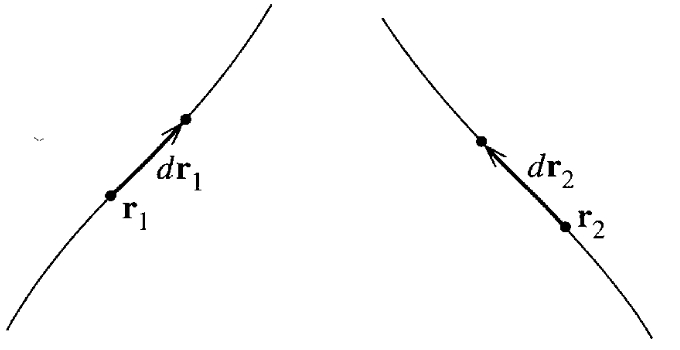
\includegraphics[width=0.5\textwidth]{CentralForcesMotion.png}
\end{figure}

We know that the toal work done will be equal to the change in kinetic energy
for each of the particles,and we can do some math to simplify that:
\begin{align*}
	W_{tot} &= \d T = \d T_1 + \d T_2\\
		&= \vec{F}_{12}\cdot\d\vec{r}_1+\vec{F}_{21}\cdot\d\vec{r}_2\\
		&= \vec{F}_{12}\cdot(\d\vec{r}_1-\d\vec{r}_2)\\
		&=\vec{F}_{12}\cdot\d(\vec{r}_1-\vec{r}_2)\\
		&= -\del_1U(\vec{r}_1-\vec{r}_2)\cdot\d(\vec{r}_1-\vec{r}_2)
\end{align*}

This result is \emph{exactly} what we got for a single particle, just with
$\vec{r} = \vec{r}_1-\vec{r}_2$.
Since we just showed the relationship between the changes in kinetic energy and
the change in potential energy, we can use that to show that the total change
in energy will always be 0 in this case, so energy will be conserved.
\[
	E \equiv T_1+T_2+U_{12}
\]


\subsubsection{Energy in \emph{N}-Particle Systems}

Kinetic energy for an $N$-particle system is easily scalable:
\[
	T = \sum_{\alpha=1}^{N}T_{\alpha}
\]

If there's no external forces, then the total potential energy,
$U^{int}$, must be taken for each set of particles, so it is
\[
	U^{int} = \sum_{\alpha=1}^{N}\sum_{\beta=1}^{N}
	U_{\alpha\beta}(\vec{r}_{\alpha}-\vec{r}_{\beta})
\]
If there is a net external force, we would also want to add
\[
	U^{ext} = \sum_{\alpha=1}^{N} U_{\alpha}^{ext}
\]

That means that
\begin{align*}
	U &= U^{int} + U^{ext}\\
	  &= \sum_{\alpha=1}^{N}\sum_{\beta=1}^{N}U_{\alpha\beta}
		(\vec{r}_{\alpha}-\vec{r}_{\beta}) + 
		\sum_{\alpha=1}^{N} U_{\alpha}^{ext}\\
	F_{\alpha} &= -\del_x\left[U_{\alpha}+\sum_{\alpha\neq\beta}^{N}
		U_{\alpha\beta}(\vec{r}_{\alpha}-\vec{r}_{\beta})\right]
\end{align*}

So if we have all conservative forces,
\begin{align*}
	E &= T = U = T + U^{ext} + U^{int}\\
	  &= \sum_{\alpha=1}^{N} \frac{1}{2}m_\alpha v_\alpha^2 +
	\sum_{\alpha=1}^NU_{\alpha}^{ext} +
	\sum_{\alpha=1}^N\sum_{\beta=1}^NU_{\alpha\beta}(\vec{r}_{\alpha}-
		\vec{r}_{\beta})
\end{align*}
In rigid bodies, the internal potential energy will remain constant, so we can
analyze rigid bodies as a single object or particle.

\section{Oscillations}
\subsection{Simple Harmonic Motion (SHM)}
\subsubsection{Simple Harmonic Oscillation and Oscillators}
\begin{defi}[Simple Harmonic Motion]
	\emph{Simple harmonic motion} is periodic, symmetric motion about an
	equilibrium point with a period independent of the magnitude of the
	motion.
\end{defi}

In one dimension, we write the equations of motion using Hooke's law:
\begin{align*}
	F = m\ddot{x} &= -k(x-x_0)\\
	U &= \frac{1}{2}k(x-x_0)^2
\end{align*}

\begin{prop}
	For any potential function with one or more minimum, small
	displacements about any minimum will exhibit SHM.
\end{prop}

\begin{proof}
	If a function $U(x)$ has a minimum at $x=x_0$, then for small
	displacements, we can approximate $U(x)$ with a Taylor series:
	\begin{align*}
		U(x) \approx U(x)\bigg\lvert_{x=x_0}
		+ \frac{\d U(x)}{\d x}\bigg\lvert_{x=x_0}(x-x_0)
		+ \frac{\d^2U(x)}{\d x^2}\bigg\lvert_{x=x_0}(x-x_0)^2
	\end{align*}
	We know that $U(x_0) = U_0$ is constant.\\
	We also know that $\frac{\d U(x_0)}{\d x} = 0$ for equilibrium terms,
	so the term vanishes.\\
	We finally know that $\frac{\d^2U(x_0)}{\d x^2} > 0$ for a 
	stable equilibrium.\\
	If we define the final term as $k$, then we're left with
	\[U(x) \approx U_0+\frac{1}{2}k(x-x_0)^2\]
	which is exactly our equation for simple harmonic motion.
\end{proof}

Our equation of motion in one dimension,
\begin{align*}
	F=m\ddot{x}&=-kx\\
	\implies m\ddot{x}+kx&=0
\end{align*}
is a homogeneous, ordinary, second-order linear differential equation, meaning
it can always be solved for two linearly independent solutions with two
arbitrary constants. Given the form of the equation, we can assume a solution
like $x\sim e^{qt}$. By substituion, we can get the characteristic equation,
\begin{align*}
	mq^2 &= -k\\
	q &= \pm i \omega_0 : \omega_0 = \sqrt{\frac{k}{m}}\\
	\implies \ddot{x} &= -\omega_0^2x
\end{align*}
$\omega_0$ is usually called the ``natural frequency.''

The solutions to this differential equation can be written in a number of
different, but equivalent, ways:
\begin{align*}
	x&=C_1e^{i\omega_0t}+C_2e^{-i\omega_0t}\\
	x&=B_1\cos(\omega_0t)+B_2\cos(\omega_0t)\\
	x&=A\cos(\omega_0t-\delta)\\
	x&=\mathrm{Re}[Ae^{i(\omega_0t-\delta)}]
\end{align*}
There are a number of constants in there we want to define real quick:
\begin{align*}
	A &\to \text{Amplitude (where the turning points are}\pm A\text{)}\\
	\omega_0=\sqrt{\frac{k}{m}} &\to \text{Natural (Angular) Frequency}\\
	\delta &\to \text{Phase Shift}\\
	\tau=\frac{2\pi}{\omega_0} &\to \text{Period}
\end{align*}

For now, we'll look at the simplest one, $x= A\cos(\omega_0t-\delta)$. To fix
the constants, we need the initial conditions. As an example, let's assume that
$x(0) = x_0$ and that $\dot{x}(0) = v(0) =v_0$. THen,
\begin{align*}
	x_0 &= A\cos(\delta)\\
	v(t) &= -\omega_0A\sin(\omega_0t-\delta)\\
	\implies& v_0 = \omega_0A\sin(\delta)
\end{align*}

We can solve this system of equations to find the amplitude. I'll skip a little
math here, but if we multiply the first by $\omega_0$, square the two
equations, then add them, then that will give us an expression for $A$:
\[
	A^2 = x_0^2 + \left(\frac{v_0}{\omega_0}\right)^2
\]

\subsubsection{Energy in Simple Harmonic Motion}
We already know that if we have something like a spring-mass system (a
simple example of something approximating simple harmonic motion), the total
energy will be given by $E=T+U=\frac{1}{2}m\dot{x}^2+\frac{1}{2}kx^2$.
Is energy conserved in SHM, though? Let's look:
\begin{align*}
	&m\ddot{x}+kx=0\\
	\frac{\d E}{\d t} &= \frac{\d}{\d t}\left[\frac{1}{2}m\dot{x}^2+
	\frac{1}{2}kx^2\right]\\
	&= m\ddot{x}\dot{x}+kx\dot{x}\\
	&=\dot{x}(m\ddot{x}+kx)\\
	&=0
\end{align*}

So, we can see that yes, in idealized simple harmonic motion, energy is
conserved. If a system is motionless at the moment $t=a$, then
\[E = U(a)+\frac{1}{2}kx_{max}^2 = \frac{1}{2}kA^2\]
At any given time, then, we can relate the speed and position:
\begin{align*}
	\frac{1}{2}kA^2 &= \frac{1}{2}m\dot{x}^2+\frac{1}{2}kx^2\\
	A^2&=\frac{m}{k}\dot{x}^2+x^2\\
	   &= \left(\frac{\dot{x}}{\omega_0}\right)^2+x^2
\end{align*}


\subsection{Damped Harmonic Motion (DHM)}
\subsubsection{Damped Harmonic Oscillation and Oscillators}
SHM is fairly ubiquitous, but it's an idealized case. In reality, oscillators
would lose energy to their surroundings, which we call ``damping.'' Although
oscillators can experience both linear and quadratic drag, quadratic drag is
difficult to calculate, so we'll mostly look at linear (Stokes's) drag.

First, let's look at the equations of motion for DHM in one dimension:
\begin{align*}
	F = &m\ddot{x} = -kx-b\dot{x}\\
	    &m\ddot{x}+b\dot{x}+kx=0
\end{align*}

This is a homogeneous, ordinary, second-order linear differential equation with
constant coefficients, meaning it will have two linearly independent solutions
with two arbitrary constants, and, more importantly, it can always be solved.

So let's solve it! With our given equation of motion, we can guess a solution
like $x\sim e^{qt}$. If we plug that in, and take out the common factors,
we end up with
\begin{align*}
	mq^2+bq+k&=0\\
	q^2+\frac{4b}{2m}q+\omega_0^2&=0\\
	q^2+2\beta q + \omega_0^2&=0\\
	\implies\ddot{x}+2\beta\dot{x}+\omega_0^2x&=0
\end{align*}
Where $\beta = \frac{b}{2m}$ and $\omega_0^2 = \frac{k}{m}$, both of which have
units of 1/sec, and both of which indicate resistance to movement (ie. drag).
This means that we can find $q = \beta\pm\sqrt{\beta^2-\omega_0^2}$, and
the general solution will be
\[
	x(t) = e^{-\beta t}\left(C_1e^{t\sqrt{\beta^2-\omega_0^2}} +
	C_2e^{-t\sqrt{\beta^2-\omega_0^2}}\right)
\]

For DHM, there are three potential situations, which we'll explore separately:

\noindent\textbf{Case 1: Underdamped}
\begin{align*}\beta^2&> \omega_0^2\\
	\implies q = -\beta&\pm\sqrt{\beta^2-\omega_0^2}
\text{ is imaginary}\end{align*}
Often, we will write $q = -\beta\pm i\omega_1$, where
$\omega_1$ is the real part of the imaginary square root (that is,
$\omega_1 = \sqrt{\omega_0^2-\beta^2}$). This means that we can re-write the
general solution as
\begin{align*}
	x(t) &= e^{-\beta t}\left(C_1e^{i\omega_1t}+C_2e^{-i\omega_1t}\right)\\
	     &= Ae^{-\beta t}\cos(\omega_1t-\delta)
\end{align*}
This is almost exactly the same as normal simple harmonic motion, except the
amplitude is decaying with time. This type of motion will osccilate at
an angular frequency $\omega_1<\omega_0$. If $x_0\neq0$ and $v_0=0$, then this
will look like the following graph:

\begin{center}
\begin{tikzpicture}
	\begin{axis}
	[
	axis lines=middle,
	xlabel={$t$},
	ylabel={$x$},
	ticks=none,
	domain=0:100
	]
	\addplot[domain=75:100]{0};
	\addplot[domain=0:84.823,samples=500]{exp(-0.07*x)*cos(deg(x))};
	\addplot[domain=0:86,samples=60,dashed]{exp(-0.07*x)};
	\addplot[domain=0:86,samples=60,dashed]{-exp(-0.07*x)};
	\end{axis}
\end{tikzpicture}
\end{center}
The dashed line on the outside is called the \emph{envelope}, and is the
decaying amplitude function $Ae^{-\beta t}$.

\noindent\textbf{Case 2: Overdamped}
\begin{align*}\beta^2&> \omega_0^2\\
	\implies q = -\beta&\pm\sqrt{\beta^2-\omega_0^2}
\text{ is real}\end{align*}

In this case, the exponential term is real, so we will end up with a
non-oscillatory exponential function. We can write our equation as
\begin{align*}
	x(t) &= e^{\beta t}\left(C_1e^{t\sqrt{\beta^2-\omega_0^2}} +
	C_2e^{-t\sqrt{\beta^2-\omega_0^2}}\right)
\end{align*}
Given the same initial conditions, $x_0\neq0$ and $v_0=0$, the graph will
look like
\begin{center}
\begin{tikzpicture}
	\begin{axis}
	[
	axis lines=middle,
	xlabel={$t$},
	ylabel={$x$},
	ticks=none,
	ymax=1.5
	]
	\addplot[domain=0:50,samples=60]{exp(-0.1*x)};
	\end{axis}
\end{tikzpicture}
\end{center}

\noindent\textbf{Case 3: Critically Damped}
\begin{align*}\beta^2 &= \omega_0^2\\ \implies q = -\beta&\pm
	\sqrt{\beta^2-\omega_0^2}=-\beta
\end{align*}

The exponential term is once again real and non-oscillatory. It will look
very similar to the previous graph, but it wil reach equilibrium ($x=0$)
quicker than its overdamped counterpart.

\subsubsection{Energy in Damped Harmonic Motion}

We know that
\begin{align*}
	E&=T+U\\
	&=\frac{1}{2}m\dot{v}^2+\frac{1}{2}kx^2\\
	\implies \frac{\d E}{\d t} &=
	\frac{\d}{\d t}\left[\frac{1}{2}m\dot{x}^2+\frac{1}{2}kx^2\right]\\
	&=m\ddot{x}\dot{x}+kx\dot{x}\\
	&=\dot{x}(m\ddot{x}+kx)\\
	&=-b\dot{x}^2
\end{align*}
This means that for any damped harmonic motion, the total change in energy is
negative, so the system is losing energy.

\subsection{Driven Damped Harmonic Motion - Sinusoidal Driving Force}
\subsubsection{Damped Harmonic Motion with a Sinusoidal Driving Force}
We'll be looking at damped harmonic motion with an external sinusoidal
driving force. The equation of motion for this will look like
\begin{align*}
	m\ddot{x}+b\dot{x}+kx&=F_0e^{i\omega t}\\
			     &=F_0\cos(\omega t)+iF_0\sin(\omega t)
\end{align*}
This is a weird way of writing it, but the idea is that if we have a cosine
driving force, we'll be look at the real part of the RHS, and subsequently
the real part of the solution. Similarly, if we have a sine driving force,
we'll be looking at the imaginary part of the RHS, and subsequently the
imaginary part of the solution.

The equation of motion is a non-homogeneous, ordinary second-order linear
differential equation with constant coefficients. This means that the solution
will be the sum of a homogeneous solution and a particular solution. The
homogeneous solution (that is, the solution when the RHS is equal to zero)
will be the general damped harmonic oscillator solution from the last
section:
\[
	x_h(t) = A_he^{\beta t}\left(C_1e^{t\sqrt{\beta^2-\omega_0^2}} +
	C_2e^{-t\sqrt{\beta^2-\omega_0^2}}\right)
\]
For the particular solution, we can use an ansatz (that is, an educated guess)
and say that
\[
	x_p(t) = A_1e^{i(\omega t-\delta)}
	= A_1(\cos(\omega t-\delta)+i\sin(\omega t-\delta))
\]
Substitution into the equation of motion will give us an equation that can
be split into real and imaginary parts:
\begin{align*}
	\mathrm{Re:}&&A_1(k-m\omega^2)&=F_0\cos(\delta)&\\
	\mathrm{Im:}&&A_1(b\omega)&=F_0\sin(\delta)&
\end{align*}
We can combine these to find that
\begin{align*}
	\tan(\delta) &= \frac{b\omega}{k-m\omega^2}\\
		     &=\frac{2\beta\omega}{\omega_0^2-\omega^2}\\
	\implies
	\delta &= \arctan\left(\frac{2\beta\omega}{\omega_0^2-\omega^2}\right)
\end{align*}

We can also use these equations to find the generalized form of $A_1$:
\begin{align*}
	A_1^2(k-m\omega)^2+A_1^2(b\omega)^2 &=
		F_0^2(\cos^2(\delta)+\sin^2(\delta))\\
	A_1^2\left((k-m\omega)^2+(b\omega)^2\right) &= F_0^2\\
	A_1(\omega) &= \frac{F_0}{\sqrt{(k-m\omega)^2+(b\omega)^2}}\\
		    &= \frac{F_0}{m\sqrt{(\omega_0^2-\omega^2)^2+
		    	4\beta^2\omega^2}}
\end{align*}
This will often be written more simply as
\[
	A_1(\omega) = \frac{F_0/m}{D(\omega)^{\frac{1}{2}}}
\]
where $D(\omega)=(\omega_0^2-\omega^2)^2+4\beta^2\omega^2$.

This is everything we need to be able to find the particular solution.
If the driving force is a sine function, then we can say that
\[
	x_p(t) = A_1\sin(\omega t-\delta)
\]
and if the driving force is a cosine function,
\[
	x_p(t) = A_1\cos(\omega t-\delta)
\]
with $A_1$ and $\delta$ being the constants we just found.

The homogeneous term, or the decaying damped harmonic oscillator term, will
go to zero as $t\to\infty$, so we call it the \emph{transient term}.

The remaining particular term, after long enough, will be the only piece
determining the motion, so we call it the \emph{steady-state solution}.

We can graph an example function showing the driving force and the position
function:
\begin{center}
\begin{tikzpicture}
	\begin{axis}
	[
	axis lines=middle,
	xlabel={$t$},
	ylabel={$F(t)$},
	ticks=none
	]
	\addplot[domain=0:75,samples=500]{cos(deg(0.2*x))};
	\end{axis}
\end{tikzpicture}
\begin{tikzpicture}
	\begin{axis}
	[
	axis lines=middle,
	xlabel={$t$},
	ylabel={$x$},
	ticks=none
	]
	\addplot[domain=0:75,samples=500]{exp(-0.07*x)*cos(deg(x))+cos(deg(0.2*x))};
	\end{axis}
\end{tikzpicture}
\end{center}

$A_1$ is maximized where $\der{A_1}{\omega} = 0$:
\begin{align*}
	\der{A_1}{\omega}\bigg\rvert_{\omega=\omega_R} = \der{}{\omega}\left[
	\frac{F_0/m}{(D(\omega))^{1/2}}\right]_{\omega=\omega_R}
	= -\frac{F_0}{2m}[D(\omega)]^{-3/2}\der{D(w)}{\omega}\bigg\rvert_{
	\omega=\omega_R} = 0
\end{align*}
We know that the denominator function, $D(\omega)$ can never be 0, since that
would give us an undefined function, so for this to be true, that means
$\der{D(\omega)}{\omega}$ must instead be equal to zero:
\begin{align*}
	\der{D(\omega)}{\omega}\bigg\rvert_{\omega=\omega_R}
	&= [2(\omega_0-\omega^2)(-2\omega)+8\beta^2\omega]_{\omega=\omega_R}\\
	&= \omega_0^2-\omega_R^2+8\beta^2 = 0\\
	\omega_R &= \sqrt{\omega_0^2-2\beta^2} = \sqrt{\omega_1^2-\beta^2}
\end{align*}
This $\omega_R$, where $A_1$ is maximized is called the ``resonant frequency.''
When the system is driven at this frequency, it is operating at its maximum,
and
\[ A_1(\omega_R) = \frac{F_0}{2\beta m\omega_1} \]
In the case of weak damping (where $\beta \ll \omega$, like Barton's pendulum),
$\omega_R \approx \omega_1 \approx \omega_0$, so \(A_1(\omega_R) \approx
\frac{F_0}{2\beta m\omega_0}\). If $\omega_0^2<2\beta^2$, when no resonance
is even possible.

\subsubsection{The Phase Shift}
\[ \delta = \arctan\left(\frac{2\beta\omega}{\omega_0^2-\omega^2}\right) \]
\begin{enumerate}
	\item If $\omega \ll \omega_0$, $\delta \approx 0$, so the motion is
		\emph{in phase} with the driving force
	\item If $\omega \approx \omega_0$, $\delta \approx \frac{\pi}{2}$, so
		the motion is $90^\circ$ \emph{out of phase} with the
		driving force
	\item If $\omega \gg \omega_0$, $\delta \approx \pi$, so the motion is
		$180^\circ$ \emph{out of phase} with the driving force
\end{enumerate}

\subsubsection{Energy in the Steady-State Driven Damped Harmonic Oscillator}
If we have a driven damped harmonic oscillator in a steady state with
$F(t) = F_0\cos(\omega t)$, then we know that
\begin{align*}
	x_{ss}(t) &= A_1\cos(\omega t-\delta)\\
	\dot{x}_{ss}(t) &= -A_1\omega\sin(\omega t-\delta)
\end{align*}
The work per unit time done by the driving force can be found with
\begin{align*}
	\der{W}{t} = \der{T}{t} &= Fv = F(t)\dot{x}\\
				&= F_0\cos(\omega t)[-A_1\omega\sin(\omega t
					-\delta)]
\end{align*}
The change in energy per unit time can be found similarly:
\begin{align*}
	\der{E}{t} &= \der{T}{t} + \der{U}{t}\\
		   &= \der{}{t}\left[\frac{1}{2}m\dot{x}^2+\frac{1}{2}kx^2
			\right]\\
		   &= (m\ddot{x}+kx)\dot{x} = -b\dot{x}^2 + F(t)\dot{x} 
\end{align*}
In a steady state, the LHS averaged over a complete cycle (or period) should
b 0. That is, the energy lost by damping should be perfectly matched by the
external forced averaged over one period, or
\[ \left\langle\der{E}{t}\right\rangle = \left\langle\der{}{t}\left[
	\frac{1}{2}m\dot{x}^2+\frac{1}{2}kx^2\right]\right\rangle =
	\langle-b\dot{x}^2+F(t)\dot{x}\rangle = 0
\]
\begin{proof}
\begin{align*}
	\dot{x} &= -A_1\omega\sin(\omega t-\delta)\\
	-b\dot{x}^2+F(t)\dot{x} &=
	-b[-A_1\omega\sin(\omega t-\delta)]^2 + F_0\cos(\omega t)[-A\omega
		\sin(\omega t-\delta)]\\
	&= -bA_1^2\omega^2\sin^2(\omega t-\delta) + A_1F_0\omega\cos(\omega t)
		\sin(\omega t-\delt\\
		&= -bA_1^2\omega^2\sin^2(\omega t-\delta) + A_1F_0\omega\left[
		\cos^2(\omega t)\sin(\delta) - \frac{1}{2}\cos(2\omega t)
		\cos(\delta)\right]
\end{align*}
We know that $\langle\sin^2(\omega t)\rangle=\langle\cos^2(\omega t)\rangle=0$,
and we can find similarly that \(\left\langla\frac{\sin(2\omega t)}{2}
\cos(\delta)\right\rangle = 0\), so the average of this becomes
\begin{align*}
	\left\langle\der{E}{t}\right\rangle &=
	-\frac{1}{2}bA_1^2\omega^2+\frac{1}{2}A_1F_0\omega\sin(\delta)\\
	&= \frac{A_1\omega}{2}(-bA_1\omega+F_0\sin(\delta)) = 0
\end{align*}
Note that the final equality to zero works because the imaginary part to our
earlier solution was $A_1(b\omega)=F_0\sin\delta$.
\end{proof}

\subsection{Driven Damped Harmonic Motion - Non-Sinusoidal Periodic Driving Force}

\subsection{Driven Damped Harmonic Motion - Impulse Forces}

\section{Lagrange's Equations}

\subsection{Derivation of Lagrange's Equations}
\subsubsection{Generalized Coordinates}
If we're considering $N$ particles in $k$ dimensions, we will always need, at
most, $n\cdot k$ coordinates to find a complete solution. For example, if we
use 3-dimensional Cartesian coordinates for a system of $N$ particles, we will
need three dimensions for each of the $N$ particles, $(x_N,y_N,z_N)$, or
$3N$ coordinates. That's often more than we actually need, though. If we have
equations that relate two or more coordinates (or \emph{constraints}), then we
can subtract the number of constraints, giving us the minimum number of
required coordinates, or \emph{degrees of freedom}.
\begin{defi}[Degrees of Freedom]
	The \emph{degrees of freedom} for a system are the minimum number 
	of coordinates needed to totally define the system, given by
	\[ f = n\cdot k - c \]
	where $n$ is the number of particles, $k$ is the number of coordinates,
	and $c$ is the number of constraints.
\end{defi}
Once we have the degrees of freedom, applying the constraints, what we're left
with will be the \emph{generalized coordinates}. There can be multiple sets of
generalized coordinates (eg. we can represent a system in either Cartesian or
polar coordinates), but they can all be expressed in $f$ coordinates.

\paragraph{Transformations between Coordinates}
Specifically, we'll be looking at transformations between Cartesian coordinates
and other potential generalized coordinates. To start, we will define
\[
	\{x_j\} = \{x_1,x_2,x_3,x_4,x_5,x_6,\ldots,x_{3N}\}
	= \{x_1,y_1,z_1,x_2,y_2,z_2,\ldots,z_N\}
\]
Now, if we want to go from $\{x_j\}$ to $\{q_k\}$, then we write
\begin{align*}
	\d x_j &= \sum_{k=1}^{f}\pder{x_j}{q_k}\d q_k\\
		\dot{x}_j&=
		\sum_{k=1}^{f}\left[\pder{x_j}{q_k}\pder{q_k}{t}\right]
			+ \pder{x_j}{t}
\end{align*}
Noting that the only time $\pder{x_j}{t}$ appears is in a moving coordinate
system.
The infinitesimals are then written as
\[
	\delta x_j = \sum_{k=1}^{f}\pder{x_j}{q_k}\delta q_k
\]

\subsubsection{Generalized Kinetic Energy}
In Cartesian coordinates, we know that
\[
	T = \frac{1}{2}\sum_{i=1}^{n}m_i(\dot{x}_i^2+\dot{y}_i^2+\dot{z}_i^2)\\
\]
Using our just-developed expression to convert between Cartesian and
generalized coordinates, we can write this as
\begin{align*}
	T =
	\sum_{k=1}^{3n}\sum_{\ell=1}^{3n}
		\left[\frac{1}{2}A_{k\ell}\dot{q}_k\dot{q}_\ell\right]
	+ \sum_{k=1}^{3n}[B_k + \dot{q}_k] + T_0
\end{align*}
Where $A_k$, $B_k$, and $T_0$ are defined as
\begin{align*}
	A_{k\ell} &= \sum_{i=1}^{3n}m_i
		\left[\pder{x_i}{q_k}\pder{x_i}{q_\ell}
		+\pder{y_i}{q_k}\pder{y_i}{q_\ell}
		+\pder{z_i}{q_k}\pder{z_i}{q_\ell}\right]\\
	B_{k} &=\sum_{i=1}^{n}m_i
		\left[\pder{x_i}{t}\pder{x_i}{q_k}
		+\pder{y_i}{t}\pder{y_i}{q_k}
		+\pder{z_i}{t}\pder{z_i}{q_k}\right]\\
	T_0 &= \sum_{i=1}^{n}\frac{1}{2}m_i
		\left[\left(\pder{x_i}{t}\right)^2
		+\left(\pder{y_i}{t}\right)^2
		+\left(\pder{z_i}{t}\right)^2\right]
\end{align*}
If $A_{k\ell}$ is nonzero only when $k=1$, then $\{q_k\}$ are orthogonal.
If the generalized coordinates don't contain explicit functions of time, we
call them ``scleronomic'' and the terms $B_k$ and $T_0$ go away. Otherwise,
they're called ``rheonomic.''

\subsubsection{Generalized Momentum}
The momentum of a single particle in the $x$ direction is
\[
	p_x = \pder{T}{\dot{x}}=m\dot{x}
\]
Similarly, for a system,
\[
	p_x = \sum_{i=1}^{n}\pder{T}{\dot{x}_i}
\]
And for a system in generalized coordinates,
\[
	p_k = \sum_{k=1}\pder{T}{\dot{q}_k}
\]

\subsubsection{Generalized Forces}
To talk about generalized forces, we first want to talk about work. Work is
generally defined as
\begin{align*}
	W &= \int\vec{F}\cdot\d\vec{r}\\
	\delta W &= \sum_{i=1}^n(F_{ix}\delta x_i + F_{iy}\delta y_i
		+ F_{iz}\delta z_i)
\end{align*}
We know from earlier that we can re-write the differential of $x_i$ in
terms of generalized coordinates with
\[ \delta x_i = \sum^f_{k=1}\pder{x_i}{q_k}\delta q_k \]
This means that we can write the differential of the work function as
\begin{align*}
	\delta W &= \sum^n_{i=1}\left[
		F_{ix}\sum^f_{k=1}\pder{x_i}{q_k}\delta q_k+
		F_{iy}\sum^f_{k=1}\pder{y_i}{q_k}\delta q_k+
		F_{iz}\sum^f_{k=1}\pder{z_i}{q_k}\delta q_k\right]\\
	\delta W &= \sum^f_{k=1}Q_kq_k
\end{align*}
This, of course, implies that
\[
	Q_k = \sum^n_{k=1}\left(F_{ix}\pder{x_i}{q_k} + F_{iy}\pder{y_i}{q_k}
	+F_{ix}\pder{x_i}{q_k}\right)
\]
What else do we know about work, though? Well, if we're working with only
conservative forces, we know that
\begin{align*}
	\delta W &= -\delta U\\
		 &= -\sum_{i=1}^n\left(\pder{U}{x_i}\delta x_i
			+\pder{U}{y_i}\delta y_i
			+\pder{U}{z_i}\delta z_i\right)\\
			&= -\sum_{i=1}^n\left(
			\pder{U}{x_i}\sum_{k=1}^f\pder{x_i}{q_k}\delta q_k
			+\pder{U}{y_i}\sum_{k=1}^f\pder{x_i}{q_k}\delta q_k
			+\pder{U}{z_i}\sum_{k=1}^f\pder{x_i}{q_k}\delta q_k
			\right)\\
		 &= -\sum_{i=1}^n\sum_{k=1}^f\left(
			\pder{U}{x_i}\pder{x_i}{q_k}\delta q_k+\cdots\right)\\
	\delta U_k &= \pder{U}{q_k}\delta q_k
\end{align*}
We can combine these things we know about the differential for work and say
that for conservative forces,
\begin{align*}
	\delta W_k = Q_k\delta q_k  &= \delta U_k = -\pder{U}{q_k}\delta q_k\\
	\implies Q_k &= -\pder{U}{q_k}
\end{align*}

If we have a mixture of conservative and non-conservative forces, this doesn't
work exactly, but it's pretty close:
\[ Q_k = \underbrace{Q'_k}_{\text{Non-Conservative}}
	-\underbrace{\pder{U}{q_k}}_{\text{Conservative}} \]

\subsubsection{Lagrange's Equations}
We know from Newton's second law that 
\[ \vec{F} = \frac{\d \vec{p}}{\d t} \]
We also know that we defined the generalized momentum as
\[ p_k = \pder{T}{\dot{q}_k} \]
Combining the two of those, we can find some interesting and useful
expressions,
and by extension, start to really develop a useful set of equations for
Lagrangian dynamics. This is pretty easy in Cartesian coordinates:
\begin{align*}
	T&=\frac{1}{2}\sum_{i=1}^{N}m_i(\dot{x}_i^2+\dot{y}_i^2+\dot{z}_i^2)\\
	\pder{T}{\dot{q}_k} &= \sum_{i=1}^{N}
		m_i\left(\dot{x}_i\pder{\dot{x}_i}{\dot{q}_k} +
			\dot{y}_i\pder{\dot{y}_i}{\dot{q}_k} +
			\dot{z}_i\pder{\dot{z}_i}{\dot{q}_k}\right)
\end{align*}

We have a definition for $\dot{x}_i$,
\[ \dot{x}_i = \sum_{k=1}^f \pder{x_i}{q_k}\dot{q}_k + \pder{x_i}{t} \]
If we take the partial of that with respect to $\dot{q}_k$, we can find that
\[ \pder{\dot{x}_i}{\dot{q}_k} = \pder{x_i}{q_k} \]
If we plug this in for the partial of $T$ with respect to
$\dot{q}_k$, and take the time-derivative to find the generalized momentum:
\begin{align*}
	\frac{\d}{\d t}\left[\pder{T}{\dot{q}_k}\right] &=
		\sum_{i=1}^N m_i\left(
			\ddot{x}_i\pder{x_i}{q_k}+
			\ddot{y}_i\pder{y_i}{q_k}+
			\ddot{z}_i\pder{z_i}{q_k}\right)\\
			&+\sum_{i=1}^Nm_i\left(
			\dot{x}_i\frac{\d}{\d t}\left[\pder{x_i}{q_k}\right]+
			\dot{y}_i\frac{\d}{\d t}\left[\pder{y_i}{q_k}\right]+
			\dot{z}_i\frac{\d}{\d t}\left[\pder{z_i}{q_k}\right]
		\right)
\end{align*}
That's a lot. But we do know that the first term of that equation is
\begin{align*}
	\sum_{i=1}^N m_i\left(
		\ddot{x}_i\pder{x_i}{q_k}+
		\ddot{y}_i\pder{y_i}{q_k}+
		\ddot{z}_i\pder{z_i}{q_k}\right)
	=\sum_{i=1}^N
		F_{ix}\pder{x_i}{q_k}+F_{iy}\pder{y_i}{q_k}+
			F_{iz}\pder{z_i}{q_k} = Q_k
\end{align*}
To solve the second part, we can remember that the order of differentiation
isn't actually important, so we can write
\begin{align*}
	\dot{x}_i\frac{\d}{\d t}\left[\pder{x_i}{q_k}\right] =
	\dot{x}_i\frac{\d}{\d q_k}\left[\pder{x_i}{t}\right] =
	\dot{x}_i\pder{\dot{x}_i}{q_k}
\end{align*}
So, putting this in the bigger part of this equation,
\begin{align*}
	&\sum_{i=1}^Nm_i\left(
	\dot{x}_i\frac{\d}{\d t}\left[\pder{x_i}{q_k}\right]+
	\dot{y}_i\frac{\d}{\d t}\left[\pder{y_i}{q_k}\right]+
	\dot{z}_i\frac{\d}{\d t}\left[\pder{z_i}{q_k}\right]\right)\\
	=&\sum_{i=1}^Nm_i\left(
	\dot{x}_i\pder{\dot{x}_i}{q_k}
	\dot{y}_i\pder{\dot{y}_i}{q_k}
	\dot{z}_i\pder{\dot{z}_i}{q_k}
	\right) = \pder{T}{q_k}
\end{align*}
Putting those two together, we get \emph{Lagrange's Equation}:
\begin{align*}
	\frac{\d}{\d t}\left[\pder{T}{\dot{q}_k}\right] &= Q_k+\pder{T}{q_k}\\
	\implies 
	\frac{\d}{\d t}\left[\pder{T}{\dot{q}_k}\right]-\pder{T}{q_k} &= Q_k
\end{align*}
If we're working with all conservative forces, so that we can write
$Q_k = -\pder{U}{q_k}$, then we can instead write
\[ \frac{\d}{\d t}\left[\pder{T}{\dot{q}_k}\right]-\pder{T}{q_k} =
	-\pder{U}{q_k} \]
But we can make this even better. If the potential isn't defined in terms of
velocity, then we define what we call the \emph{Lagrangian}, $\mathcal{L}$:
\[ \mathcal{L} = T - U \]
If we use this definition in Lagrange's equation, we get the Euler-Lagrange
Equation for, respectively, non-conservative and conservative forces:
\begin{align*}
	\frac{\d}{\d t}\left[\pder{\mathcal{L}}{\dot{q}_k}\right]
	-\pder{\mathcal{L}}{q_k} &= Q_k'\\
	\frac{\d}{\d t}\left[\pder{\mathcal{L}}{\dot{q}_k}\right]
	-\pder{\mathcal{L}}{q_k} &= 0\\
\end{align*}

These sets of equations are applicable to any set of generalized coordinates.
Note that Lagrange's Equation requires no reatructions on $U$, while
the Euler-Lagrange Equation does. In general, we can define a problem-solving
strategy using this definition of Lagrangian dynamics.

\tikzstyle{block} = [rectangle, draw, text width=8em, text centered,
rounded corners, minimum height=4em]
\tikzstyle{block1} = [rectangle, draw, text width=11em, text centered,
rounded corners, minimum height=4em]
\tikzstyle{line} = [draw, -latex']
\begin{center}
\begin{tikzpicture}[node distance = 9em, auto]
	\node [block1] (one) {Identify degrees of freedom,\\$f=nk-c$,\\and
		choose a set of generalized coordinates};
	\node [block1, below of=one] (two) {Write the kinetic energy, $T$, in
			terms of the generalized coordinates $q_k$ and/or their
		time derivatives};

	\node [block, below of=two] (threec) {Find the potential,
		$U(q_k)$, in terms of generalized coordinates};
	\node [block, below of=threec] (fourc) {Find $Q_k'$};
	\node [block, below of=fourc] (fivec) {Construct Lagrangian
		$\mathcal{L}$};
	\node [block, below of=fivec] (sixc) {Substitute $Q_k'$ and
		$\mathcal{L}$ into the Euler-Lagrange equation};
	\node [block, below of=sixc] (sevenc) {Solve the $f$ differential
		equations};

	\node [block, left of=threec] (threea) {Find the potential, $U$, in
		terms of generalized coordinates};
	\node [block, below of=threea] (foura) {Construct the Lagrangian
		$\mathcal{L} = T - U$};
	\node [block, below of=foura] (fivea) {Substitute $\mathcal{L}$ into
		the Euler-Lagrange Equation};
	\node [block, below of=fivea] (sixa) {Solve the $f$ differential
		equations};

	\node [block, right of=threec] (threeb) {Find $Q_k$ for each force};
	\node [block, below of=threeb] (fourb) {Plug $T$ into Lagrange's
		Equation};
	\node [block, below of=fourb] (fiveb) {Solve the $f$ differential
		equations};

	\path [line] (one) -- (two);
	\path [line] (two) -- (threea)
		node [node distance = 5em, above of=threea] {All conservative};
	\path [line] (threea) -- (foura);
	\path [line] (foura) -- (fivea);
	\path [line] (fivea) -- (sixa);
	\path [line] (two) -- (threeb)
		node [node distance = 5em, above of=threeb] {All non-conservative};
	\path [line] (threeb) -- (fourb);
	\path [line] (fourb) -- (fiveb);
	\path [line] (two) -- (threec)
		node [node distance=5em, above of=threec] {Mixture};
	\path [line] (threec) -- (fourc);
	\path [line] (fourc) -- (fivec);
	\path [line] (fivec) -- (sixc);
	\path [line] (sixc) -- (sevenc);
\end{tikzpicture}
\end{center}

\subsection{Applications of Lagrange's Equations}
\subsubsection{Elementary Examples}
For these first few elementary examples, we will deal exclusively with
conservative forces.

\begin{enumerate}[label=\arabic*.]
	\item Find the equations of motion for a one-dimensional
		mass-spring system with mass $m$ and spring constant $k$.
		\begin{enumerate}[label=\roman*.]
		\item Identify the degrees of freedom\\
			There is one ``particle'' (the mass), moving in one
			dimension, and there are no constraints on that
			movement, so $n = 1$, $k = 1$, and $c = 0$, meaning
			$f = nk-c = 1$. We can choose this coordinate
			to be anything, but it's probably easiest to choose it
			as $x$.
		\item Write the kinetic energy in terms of generalized
			coordinates
			\[ T = \frac{1}{2}m\dot{x}^2 \]
		\item All forces are conservative, so find the potential
			in terms of generalized coordinates
			\[ U = \frac{1}{2}kx^2 \]
		\item Construct the Lagrangian
			\[ \mathcal{L} = T - U = \frac{1}{2}m\dot{x}^2 -
			\frac{1}{2}kx^2 \]
		\item Substitute into the Euler-Lagrange equation
			\[
				\frac{\d}{\d t}\left[\pder{\Lp}{\dot{q}_k}
				\right] - \pder{\Lp}{q_k} = 0
			\]
			\begin{align*}
				\pder{\Lp}{\dot{x}} = \pd{\dot{x}}
				\left[\frac{1}{2}m\dot{x}^2-\frac{1}{2}k
				x^2\right]
				&= m\dot{x}\\
				\frac{\d}{\d t}\left[\pder{\Lp}{\dot{x}}\right]
				=\frac{\d}{\d t}\left[m\dot{x}\right]
				&=m\ddot{x}\\
				\pder{\Lp}{x} = \pd{x}\left[\frac{1}{2}
				m\dot{x}^2-\frac{1}{2}kx^2\right]
				&= -kx\\
			\end{align*}
			\[
				\frac{\d}{\d t}\left[\pder{\Lp}{\dot{q}_k}
				\right] - \pder{\Lp}{q_k} =
				m\ddot{x}+kx = 0
			\]
		\item Solve the differential equation\\
			As we saw in chapter 5, we can solve this by
			\[ x(t) = A\cos(\omega t - \delta) \]
			where $\omega = \sqrt{k/m}$ and $A$ and $\delta$ are
			fixed by the initial conditions.
		\end{enumerate}
	\item Find the equation(s) of motion for a simple pendulum of length
		$\ell$ and mass $m$.
	\begin{enumerate}[label=\roman*.]
		\item Identify degrees of freedom\\
			There is, one particle, the mass, moving
			now in two dimensions ($x$ and $y$), but now
			there is also an extra constraint: the distance
			from the rotation point to the mass must always
			be $\ell$. Therefore, the degrees of freedom
			are equal to $f=nk-c=1$. We will use $\theta$,
			the angle the mass and string make with the
			vertical, for our generalized coordinate.
		\item Write the kinetic energy in terms of the
			generalized coordinate
			\[ T = \frac{1}{2}mv^2 = \frac{1}{2}m
				(\ell\dot{\theta})^2=\frac{1}{2}
				m\ell^2\dot{\theta}^2 \]
		\item All forces are conservative, so find the
			potential in terms of general coordinates
			\[ U = mgl(1-\cos\theta) \]
			\textit{(Gravitational potential energy)}
		\item Construct the Lagrangian
			\[ \Lp = T-U = \frac{1}{2}m\ell^2\dot{\theta}^2
			-mg\ell(1-\cos\theta) \]
		\item Substitute into the Eurler-Lagrange equation
			\[
				\frac{\d}{\d t}\left[\pder{\Lp}{\dot{q}_k}
				\right] - \pder{\Lp}{q_k} = 0
			\]
			\begin{align*}
				\pder{\Lp}{\dot{\theta}}&=m\ell^2\dot{\theta}\\
				\frac{\d}{\d t}\left[\pder{\Lp}{\dot{\theta}}
					\right] &= m\ell^2\ddot{\theta}\\
				\pder{\Lp}{\theta} &= -mg\ell\sin\theta
			\end{align*}
			\[
				\frac{\d}{\d t}\left[\pder{\Lp}{\dot{q}_k}
				\right] - \pder{\Lp}{q_k} =
				m\ell^2\ddot{\theta}+mg\ell\sin\theta=0
			\]
		\item Solve the differential equation
			\begin{align*}
				m\ell^2\ddot{\theta} &= -mg\ell\sin\theta\\
				\ell\ddot{\theta} &= -g\sin\theta\\
			\end{align*}
			For small $\theta$ values,
			\begin{align*}
				\ell\ddot{\theta} &= -g\theta\\
				\theta(t) &= A\cos(\omega t-\delta)
			\end{align*}
			where $\omega = \sqrt{g/\ell}$
	\end{enumerate}
\end{enumerate}

\subsubsection{Ignorable Coordinates}
When we're looking at situations involving central forces, we often want to
use spherical polar coordinates. We have an expression for kinetic energy in
generalized coordinates that we can apply to SP coordinates specifically:
\begin{align*}
	T &= \sum_{k=1}^{3n}\sum_{\ell=1}^{3n}\frac{1}{2}A_{k\ell}
		\dot{q}_k\dot{q}_\ell +
		\sum_{k=1}^{3n}B_k\dot{q}_k+T_0
\end{align*}
The last two terms we said would only appear if we had a coordinate system that
was changing in time, which we generally don't with SP coordinates, so they can
be ignored. Using that general form, with expressions from the metric tensor
for SP coordinates:
\begin{align*}
	T = \frac{1}{2}m(\dot{r}^2 + r^2\dot{\theta}^2 +
		r^2\sin^2\theta\dot{\varphi}^2)
\end{align*}

The potential energy we can't know generally, so we'll just call it
$U(r,\theta,\varphi)$ for now, with the note that if we're working with
central forces, it'll be $U(r)$. That means we have everything we need to
write a general version of the Lagrangian in SP coordinates:
\[
	\Lp = T-U
	= \frac{1}{2}m(\dot{r}^2 + r^2\dot{\theta}^2 +
	r^2\sin^2\theta\dot{\varphi}^2) - U(r,\theta,\varphi)
\]

As an aside, we have defined the generalized momentum as
\[ p_k = \pder{T}{\dot{q}_k} \]
Alternatively, if we follow some textbooks and assume that the potential energy
function has no explicit velocity or time dependence, then we can say
equivalently that
\[ p_k = \pder{\Lp}{\dot{q}_k} \]
If we decide to use this definition of momentum, then we can re-write the
Euler-Lagrange equation:
\begin{align*}
	\frac{\d}{\d t}\left[\pder{\Lp}{\dot{q}_k}\right]-\pder{\Lp}{q_k} &=0\\
	\frac{\d}{\d t}\left[\pder{\Lp}{\dot{q}_k}\right]&=\pder{\Lp}{q_k}\\
	\frac{\d p_k}{\d t} &= \pder{\Lp}{q_k}
\end{align*}

Why is this important? It makes this next section a lot more clear. If
the time derivative of momentum is equal to zero (and thus its implied values
are equal to zero), then\ldots there is no changeing momentum, and therefore
no changing velocity, so there's no net force or acceleration in that
direction! We call any coordinate for which this is true ``ignorable.''
That name is a little bit misleading, because we don't actually want to totally
ignore it, but it's not really that important when we're developing our
equations of motion, because there is always constant velocity. Why did we
spend so much time developing the Lagrangian for SP coordinates just to talk
about ignorable coordinates? Let's see!

Using the Lagrangian we constructed for SP coordinates earlier, if we try
to find the EOMs for each of the three coordinates, we get some interesting
results.\\
For $r$:
\begin{align*}
	\frac{\d}{\d t}\left[\pder{\Lp}{\dot{r}}\right] &=
	\frac{\d p_r}{\d t} = \frac{\d}{\d t}\left[m\dot{r}\right]= m\ddot{r}\\
	m\ddot{r} &= \pder{\Lp}{r} = mr\dot{\theta}^2+mr\sin^2\theta
	\dot{\varphi}^2-\pder{U}{r}
\end{align*}
For $\theta$:
\begin{align*}
	\frac{\d}{\d t}\left[\pder{\Lp}{\dot{\theta}}\right] &=
	\frac{\d}{\d t}[p_\theta] = \frac{d}{\d t}[mr^2\dot{\theta}]\\
	\frac{d}{\d t}[mr^2\dot{\theta}] &= m(2r\dot{r}\dot{\theta} +
	r^2\ddot{\theta}) = \pder{\Lp}{\theta} = mr^2\sin\theta\cos\theta
	\dot{\varphi}^2-\pder{U}{\theta}
\end{align*}
For $\varphi$:
\begin{align*}
	\frac{\d}{\d t}[mr^2\sin^2\theta\dot{\varphi}]=
	\pder{\Lp}{t} = -\pder{U}{\dot{\varphi}}
\end{align*}
This doesn't tell us that much on its surface. But, if we have exclusively
central forces, it does tell us something important. Recall that central forces
imply that $U = U(r)$, so in that case, $\pder{U(r)}{\dot{\varphi}}$ would
vanish, meaning
\[ \pder{\Lp}{t} = \pder{p_{\varphi}}{t} = 0 \]
This makes $\varphi$ an ignorable coordinate!

\subsubsection{Electromagnetic Forces and Velocity-Dependent Potentials}

\section{Two-Body, Central-Force Motion}

\section{Mechanics in Non-Intertial Frames}
\subsection{Basic Equations for Non-Inertial Reference Frames}

\subsubsection{Definitions and Standards}
\begin{defi}[Reference Frame]
	A \emph{reference frame} is a choice of coordinate axes by which the
	position and motion of an object can be specified.
\end{defi}
\begin{defi}[Inertial Reference Frame]
	An \emph{inertial reference frame} (IRF) is a reference frame in which
	Newton's first law (the law of inertia, ``in the absence of external
	forces, a particle moves with constant velocity'') holds.
	Generally, this is a non-rotational reference frame moving at a
	onstant velocity (including 0).
\end{defi}
\begin{defi}[Non-Inertial Reference Frame]
	A \emph{non-inertial reference frame} (NIRF) is a reference frame in
	which Newton's first law does not hold. Generally, this is a
	rotating or accelerating reference frame.
\end{defi}

For the purposes of this chapter (and the remainder of this class), we'll
follow Taylor and go against many other textbooks by using primes to refer to
IRFs, and normal coordinates to refer to NIRFs. So, for example,
$\vec{v}'$ would describe the velocity of a particle in an IRF, whereas 
$\vec{v}$ would describe the velocity of a particle in a NIRF.

\subsubsection{Translational Motion Between Reference Frames}
Consider two reference frames: one stationary IRF, $S'$, and one
accelerating NIRF, $S$, whose origin is a distance $\vec{R}'$ from the origin
of $S'$, moving at a rate of $\vec{V}'$ with respect to the origin of $S'$.

\noindent
A particle, $P$ can be measured at $\vec{r}$ in the $S$ frame, or at
$\vec{r}'$ in the $S'$ frame. Based on the figure, we can say that
\begin{align*}
	\vec{r}'&=\vec{R}'+\vec{r} &\implies& \vec{r'}-\vec{R}'=\vec{r}\\
	\vec{v}'&=\vec{V}'+\vec{v} &\implies& \vec{v'}-\vec{V}'=\vec{v}\\
	\vec{a}'&=\vec{A}'+\vec{a} &\implies& \vec{a'}-\vec{A}'=\vec{a}
\end{align*}

If Newton's second law holds in the NIRF(and we assume that it always does),
then
\begin{align*}
	\vec{F} = m\vec{a} &= m(\vec{a}'-\vec{A}')\\
			   &= m\vec{a}'-m\vec{A}'\\
			   &= m\vec{a}'+\vec{F}_{inertial}
\end{align*}
Where $\vec{F}_{inertial} = -m\vec{A}'$ is called the
``fictitious,'' ``pseudo,'' or ``apparent'' force.

\subsubsection{Rotational Motion Between Reference Frames}
Consider two frames, $S$ and $S'$, with the same origin, but $S$ is rotating
about an axis $\hat{\vec{u}}$,
with an angular velocity of $\vec{\Omega}'$ with respect to the $S'$ frame.
Since the origins coincide, and there is no translational motion,
$\vec{R}'=0$, $\vec{V}'=0$, $\vec{A}'=0$, and for some particle $P$,
$\vec{r}=\vec{r}'$.
From this, we can derive the expressions
\begin{align*}
	\frac{\d\vec{r}}{\d t} = \frac{\d\vec{r}'}{\d t} = \vec{v}' &=
	\frac{\d}{\d t}\left[x\x+y\y+z\z\right]\\
	&= \der{x}{t}\x+\der{y}{t}\y+\der{z}{t}\z+x\der{\x}{t}+y\der{\y}{t}+
		z\der{\z}{t}\\
	&= \vec{v} + x\der{\x}{t}+y\der{\y}{t}+z\der{\z}{t}
\end{align*}

\begin{center}
\begin{tikzpicture}
	\draw[->] (-2,-1.5) -- (2,1.5) node [above right] {$\vec{\Omega}$};
	\draw (0,0) circle ({2/3});
	\draw (0,0) arc [radius=1,start angle=45, end angle=120];
\end{tikzpicture}
\end{center}

In a time $\d t$, $\x$ changes by $\d\x$, such that
\[ \lvert\d\x\rvert\approx\lvert\x\rvert\Omega\sin\alpha\d t \]
Where $\approx$ becomes $=$ if we take $\d t$ to be infinitesimally small.
By extension,
\begin{align*}
	\left\lvert\frac{\d\x}{\d t}\right\rvert &= \Omega\sin\alpha\\
	\left\lvert\frac{\d\x}{\d t}\right\rvert &= \vec{\Omega}\times\x
\end{align*}
We can expand this to more than juust $\x$ and use this result to simplify the
expression we found earlier for $\frac{\d\vec{r}}{\d t}$:
\begin{align*}
	\frac{\d\vec{r}'}{\d t} &= \vec{v} + \vec{\Omega}\times\left[
		x\x+y\y+z\z\right]\\
		&= \vec{v}+\vec{\Omega}\times\vec{r}
\end{align*}
This is super important because \emph{any} vector can be written this way!
\begin{thm}[Coriolis's Theorem]
	Any arbitrary vector $\vec{Q}'$ in the IRF can be written in the NIRF
	as
	\[\frac{\d\vec{Q}'}{\d t}=\frac{\d\vec{Q}}{\d t}+\Omega\times\vec{Q}\]
\end{thm}

To convert forces between the frames, we start with the fact that in the IRF,
we know that Newton's second law must hold, so
\[ \vec{F}' = m\vec{a}' = m\frac{\d\vec{v}'}{\d t} \]
Using the Coriolus theorem, we can find that
\begin{align*}
	\vec{a}' = \der{\vec{v}'}{t} &= \frac{\d}{\d t}[\vec{v}+\vec{\Omega}
	\times\vec{r}]+\vec{\Omega}\times(\vec{v}+\Omega\times\vec{r})\\
	\vec{a}' &= \vec{a} + \left(\der{\Omega}{t}\times\vec{r}\right)
	+\left(\vec{\Omega}\times\der{\vec{r}}{t}\right)+(\vec{\Omega}\times
	\vec{v}) + \vec{\Omega}\times(\vec{\Omega}\times\vec{r})
\end{align*}
Putting this into the definition of a force, this means that
\begin{align*}
	\vec{F}' &= m\vec{a}'\\
		 &= \vec{F} - m(\dot{\vec{\Omega}}\times\vec{r}) - 2m(
		\vec{\Omega}\times\vec{v}) - m\vec{\Omega}\times(
		\vec{\Omega}\times\vec{r})
\end{align*}
Where every term after the $\vec{F}$ is called a ``fictitious force,'' and
specifically:
\begin{enumerate}
	\item \(-m(\dot{\vec{\Omega}}\times\vec{r})\) is called the
		``transverse force,'' and is zero unless the rotational
		velocity is changing.
	\item \(-2m(\vec{\Omega}\times\vec{v})\) is called the ``Coriolis
		force,'' and is zero unless the particle moves in the
		NIRF
	\item \(-m\vec{\Omega}\times(\vec{\Omega}\times\vec{r})\) is called the
		``centrifugal force,'' and is the force due to the presence
		of the rotation of the NIRF.
\end{enumerate}

\subsubsection{General Motion Between Reference Frames}
We've seen how to convert motion where the NIRF has only translational motion,
and where the NIRF has only rotational motion, so if we want to know how to
examine one with both, we can just add those together to get the \emph{very}
important result:
\[ \vec{F} = \vec{F}'-m\vec{A}'-m(\dot{\vec{\Omega}}\times\vec{r}) -
	2m(\vec{\Omega}\times\vec{v})-m\vec{\Omega}\times(\vec{\Omega}\times
	\vec{r}) \]

\subsection{Motion in a Non-Intertial Reference Frame: The Earth}
\subsubsection{Considerations for Earth as a Non-Inertial Reference Frame}
\begin{enumerate}
	\item The Earth rotates about its axis at an angular velocity of
		$\Omega_E = \frac{2\pi}{85164}\mathrm{s^{-1}}$
		$= 7.29\times10^{-5} \mathrm{s^{-1}}$
	\item For the purposes of this problem, $\Omega_E^2 = 5.3\times10^{-9}$
		is small enough to be ignorable
	\item Similarly, the Earth's rotational angular momentum doesn't change
		enough for us to care about it right now, so we can consider
		it ignorable
	\item Two products show up quite a bit so it's nice to have them
		recorded here and now:
		\begin{align*}
			\Omega_E R_E &= 464 \mathrm{m\cdot s^{-1}}\\
			\Omega_E R_E^2 &= 3.4\times 10^{-3} \mathrm{g}
		\end{align*}
\end{enumerate}

\subsubsection{The Plumb Line (and the Centrifugal Force)}
\begin{defi}[Plumb line]
	A \emph{plumb line} is a tool resembling a pendulum that is used to
	find the ``local vertical.''
\end{defi}
Problem setup:
\begin{itemize}
	\item Inertial reference frame: The origin at th center of the Earth,
		the $\z'$ axis pointing out the north pole
	\item Non-inertial reference frame: The origin at the surface of the
		Earth at a colatitude (angle from $\z'$) of $\theta$,
		the $\z$ axis pointing up the local vertical, and the
		$\y$ axis pointing north
\end{itemize}
Since the bob of the plumb line is relatively stationary, $\vec{v}=0$, and
the term $m(\vec{\Omega}\times\vec{v})=0$.\\
Earth's angular velocity will have components along both the $\y$ and $\z$
axes, so in the NIRF,
\[ \vec{\Omega}_E = \begin{pmatrix}0\\\Omega\sin\theta\\
	\Omega\cos\theta\end{pmatrix} \]

The NIRF force equation then becomes
\begin{align*}
	m\ddot{\vec{r}} &= \vec{F}'-m\vec{\Omega}\times(\vec{\Omega}\times
	\vec{r})\\
	m\vec{g} &= m\vec{g}' - m\vec{\Omega}\times(\vec{\Omega}\times\vec{r})
\end{align*}
Examining some of these individually, $\vec{g}'=9.81 \mathrm{m\cdot s^{-1}}$
points towards th center of the Earth. $\vec{g}$, however, is the overall
NIRF acceleration which includes both $\vec{g}'$ and the acceleration of the
centrifugal force, meaning it won't point exactly towards the center of the
Earth. Choosing spherical coordinates for our approximately-spherical Earth,
\begin{align*}
	\vec{F}_{cf} &= -m\vec{\Omega}\times(\vec{\Omega}\times\vec{r})
		= -m\Omega^2\rho\hat{\vec{\rho}}\\
	m\vec{g} &= m\vec{g}' - \vec{\Omega}\times(\vec{\Omega}\times\vec{r})\\
	\vec{g} &= \vec{g}' - \vec{\Omega}\times(\vec{\Omega}\times\vec{r})\\
	\vec{g} &= \vec{g}' + \Omega^2\rho\hat{\vec{\rho}}
\end{align*}
In a picture,
\begin{center}
\begin{tikzpicture}
	\draw [<-] (0,0) -- (3,1);
	\node at (1.5,0.75) {$\vec{g}'$};
	\draw [->] (3,1) -- (2,0);
	\node at (2.75,0.25) {$\vec{g}$};
	\draw [->] (2,0) -- (0,0);
	\node at (1.4, -0.25) {$\vec{\Omega^2\rho}$};
	\draw [domain=198:225] plot [smooth] ({3+cos(\x)},{1+sin(\x)});
	\node at (2,0.38) {$\alpha$};
	\draw [dashed] (0,0) -- (0,1.5);
	\draw [domain=18:90] plot [smooth] ({0.5*cos(\x)},{0.5*sin(\x)})
		node [above right] {$\theta$};
\end{tikzpicture}
\end{center}
Using this picture, we know from the law of sines that
\begin{align*}
	\frac{\Omega^2\rho}{\sin\alpha} &= \frac{\vec{g}}{\sin\left(
		\frac{\pi}{2}-\theta\right)}
		= \frac{\vec{g}}{\cos\theta}\\
		\sin\alpha &= \frac{\Omega^2(R_E\sin\theta)\cos\theta}
		{g} = \frac{\Omega^2R_E\sin(2\theta)}{2g}
\end{align*}
If we assume that $\vec{g} = \vec{g}'$, which is true to a few parts per
thousand, then the biggest $\alpha$ will get, at $\theta=45^\circ$, will
be is $\alpha\approx0.1^\circ$. The $\vec{F}_{cf}$ is, therefore, existant but
largely ignorable on the Earth, even at the equator (where $\theta=45^\circ$).
This means that, to a pretty accurate precision, we can simply write
$\vec{F} = \vec{F}'$ on the surface of the Earth.

\subsubsection{General Motion at the Earth's Surface (and the Coriolis Force)}
Without ignoring the Coriolis force, we know that
\begin{align*}
	m\ddot{\vec{r}} &\approx m\vec{g}-2m(\vec{\Omega}\times\vec{v})\\
	\ddot{\vec{r}} &\approx -g\z-2(\vec{\Omega}\times\vec{v})
\end{align*}
The Coriolis acceleration here is
\[ -2(\vec{\Omega}\times\vec{v}) = 2\Omega\begin{pmatrix}
	\dot{y}\cos\theta-\dot{z}\sin\theta\\
	-\dot{x}\cos\theta\\
	-\dot{x}\sin\theta
\end{pmatrix}
\]
Altogether, including the Coriolis aceleration, we can write 
\[ \ddot{\vec{r}} = \begin{pmatrix}
		2\dot{y}\Omega\cos\theta-2\dot{z}\Omega\sin\theta\\
		-2\dot{x}\Omega\cos\theta\\
		-g+2\dot{x}\Omega\sin\theta
	\end{pmatrix}
\]

\begin{eg}
	Let's say we drop a rock from the height $z=h$. Initially,
	\[ \begin{pmatrix}\dot{x}\\\dot{y}\\\dot{z}\end{pmatrix} = 
	\begin{pmatrix}0\\0\\0\end{pmatrix} \]
	We can solve the coupled equations of motion easily, but lets try a
	slightly different approach. Let's say that
	$\dot{x}=\dot{y}=0$, and $\dot{z}=-gt$. Then,
	\begin{align*}
		\ddot{\vec{r}} &=
		\begin{pmatrix}
			2gt\Omega\sin\theta\\
			0\\
			-g
		\end{pmatrix}\\
		\dot{\vec{r}} &=
		\begin{pmatrix}
			gt^2\Omega\sin\theta\\
			0\\
			-gt
		\end{pmatrix}\\
		\vec{r} &=
		\begin{pmatrix}
			\frac{1}{3}gt^3\Omega\sin\theta\\
			0\\
			h-\frac{1}{2}gt^2
		\end{pmatrix}\\
	\end{align*}
	So, in this non-inertial reference frame, when an object is dropped, it
	will move to the east by
	\[ x\approx \frac{1}{3}gt^3\Omega\sin\theta = \frac{\Omega g}{3}
	\left(\frac{2h}{g}\right)^{3/2}\sin\theta \]
\end{eg}

\subsubsection{The Foucault Pendulum}

\section{Rotational Motion of Rigid Bodies}
\subsection{Angular Momentum and Energy of a Rotating Body}
\subsubsection{General Notes on Rigid Bodies}
\begin{defi}[Rigid body]
	A \emph{rigid body} is a system of $N$ particles which retain their
	relative position with respect to each other.
\end{defi}
In a rigid body, the location of the $i$th particle is
\[ \vec{r}_i = x_i\x+y_i\y+z_i\z \]

\subsubsection{Rotation About a Fixed Axis}
If a fixed body rotates about the $z$ axis, which passes through it, with
angular velocity $\vec{\omega} = \omega\z$, then from what we've learned
before, the velocity of the $i$th particle is
\[ \vec{v}_i = \vec{\omega}\times\vec{r}_i = \begin{pmatrix}-\omega y_i\\\omega
x_i\\0\end{pmatrix}\]
The total kinetic energy of this system is then
\begin{align*}
	T &= \sum_{i=1}^{N}m_iv_i^2
	  = \sum_{i=1}^{N} \frac{1}{2}m_i(x_i^2+y_i^2)\omega^2
	  = \frac{1}{2}I_{zz}\omega^2
\end{align*}
Where $I_{zz} = \sum_{i=1}^{N} m_i(x_i^2+y_i^1)$ is called the ``moment of
inertia about the $z$ axis.'' Similarly, we can find the total angular
momentum:
\begin{align*}
	\vec{L} &= \sum_{i=1}^{N} \vec{L}_i = \sum_{i=1}^{N} \vec{r}_i\times
	m_i\vec{v}_i\\
	& = \sum_{i=1}^{N} m_i\{[-\omega z_ix_i]\x+[\omega z_iy_i]\y +
	[\omega(x_i^2+y_i^2)]\z\}\\
	&= I_{zx}\omega\x + I_{zy}\omega\y+I_{zz}\omega\z
\end{align*}
Where $I_{zx}$ and $I_{zy}$ are called ``products of inertia.'' Note that if
either (or both) of the products of inertia is not equal to zero, $\vec{L}$ is
not parallel to $\vec{\omega}$, and the direction of $\vec{L}$ will be
continuously changing unless a sufficient torque is applied.

If we have a continuous object rather than a system of $N$ objects, then we
take the integral over the mass distribution $\varrho\d m$:
\begin{align*}
	\sum_{i=1}^{N} m_i &\to \int\d m\\
	I_{zx} = -\sum_{i=1}^{N}m_i(z_ix_i) &\to
	-\int\d mzx = -\int\varrho\d Vzx
\end{align*}

\subsubsection{Rotation About an Arbitrary Axis}
If we have the same rigid body, but we decide to instead rotate about some
other arbitrary axis such that
\[ \vec{\omega} = \omega_x\x+\omega_y\y+\omega_z\z \]
To get the angular momentum of the $i$th particle, we can find
\begin{align*}
	\vec{L}_i =\ &\sum_{i=1}^{N} \vec{r}_i\times m_i\vec{v}_i
		= \vec{r}_i\times m_i(\vec{\omega}\times\vec{r}_i)\\
	=\ &m_i[(y_i^2+z_i^2)\omega_x-x_iy_i\omega_y-x_iz_i\omega_z]\x\\
	&+ m_i[-y_ix_i\omega_x + (z_i^2+x_i^2)\omega_y - y_iz_i\omega_z]\y\\
	&+ m_i[-z_ix_i\omega_x - z_iy_i\omega_y + (x_i^2+y_i^2)\omega_z]\z\\
	=\ &L_{xi}\x + L_{yi}\y + L_{zi}\z
\end{align*}
To find the total angular momentum, we would need to sum over all of these
individual angular momenta:
\begin{align*}
	\vec{L}=\ &\sum_{i=1}^{N}\vec{L}_i\\
	=\ &\left\{\left[\sum_{i=1}^{N}m_i(y_i^2+z_i^2)\right]\omega_x
		-\left[\sum_{i=1}^{N}m_ix_iy_y\right]\omega_y
		-\left[\sum_{i=1}^{N}m_ix_iz_i\right]\omega_z\right\}\x\\
	&+ \left\{\left[\sum_{i=1}^{N}m_iy_ix_i\right]\omega_x
		-\left[\sum_{i=1}^{N}m_i(z_i^2+x_i^2)\right]\omega_y
		-\left[\sum_{i=1}^{N}m_iy_iz_i\right]\omega_z\right\}\y\\ 
	&+ \left\{\left[\sum_{i=1}^{N}m_iz_ix_i\right]\omega_x
		-\left[\sum_{i=1}^{N}m_iz_iy_i\right]\omega_y
		-\left[\sum_{i=1}^{N}m_i(x_i^2+y_i^2)\right]\omega_z\right\}\z\\
	=\ &[I_{xx}\omega_x+I_{xy}\omega_y+I_{xz}\omega_z]\x\\
	   &+[I_{yx}\omega_x+I_{yy}\omega_y+I_{yz}\omega_z]\y\\
	   &+[I_{zx}\omega_x+I_{zy}\omega_y+I_{zz}\omega_z]\z
\end{align*}
That's a lot of work to write and it also looks a whole lot like a linear
combination that can be written as the product of a matrix and a vector.
That's good, because it is. We can write this as the product of the vector
$\vec{\omega}$ and the moment of inertia tensor, $\I$, where
\begin{align*}
	\I &=
	\begin{pmatrix}
		I_{xx} & I_{xy} & I_{xz}\\
		I_{yx} & I_{yy} & I_{yz}\\
		I_{zx} & I_{zy} & I_{zz}
	\end{pmatrix}
	,&\vec{\omega} =
	\begin{pmatrix}
		\omega_x\\
		\omega_y\\
		\omega_z
	\end{pmatrix}
\end{align*}
Note that $\I$ is diagonally symmetric and it depends on the chosen set of
axes.
I won't go through the work here, but we can use a similar process to show
that
\[ T = \frac{1}{2}\vec{\omega}\times\vec{L} = \frac{1}{2}\vec{\omega}\cdot
\I\vec{\omega} \]

As before, in the case of continuous bodies, we would replace the $I_{x_ix_j}$
terms with integrals instead of sums.

\begin{eg}
	Find $\I$ for a solid cube rotating about 1 corner. Use axes
	parallel to the cube's edge. Sides have a length $a$, the origin is
	placed at one corner. The total mass of the object is $M$, so
	$\varrho = \frac{M}{a^3}$. Find the the total angular momentum,
	$\vec{L}$, if the object is rotated about the $x$ axis, and about the
	main diagonal.\\~\\

	\begin{align*}
		I_{xx}&=\int_0^a\d x\int_0^a\d y\int_0^a\d z\varrho(y^2+z^2)\\
		      &= \frac{2\varrho a^5}{3} = \frac{2}{3}Ma^3
	\end{align*}
	The symmetry of the cube implies that $I_{xx} = I_{yy} = I_{zz}$, so
	we've successfully found the diagonal components of $\I$, or the
	moments of inertia.

	\begin{align*}
		I_{xy} = -\int\d m xy &= -\int_0^a\d x\int_0^a\d y\int_0^a\d z
		\varrho xy\\
		&=-\varrho\left(\frac{a^2}{2}\right)\left(\frac{a^2}{2}\right)\\
		&= -\frac{1}{4}Ma^2
	\end{align*}
	Similarly, symmetry implies that the other products of inertia will all
	be the same.

	So, we can write $\I$ as:
	\[
		\I = Ma^2
		\begin{pmatrix}
			2/3 & -1/4 & -1/4\\
			-1/4 & 2/3 & -1/4\\
			-1/4 & -1/4 & 2/3
		\end{pmatrix}
		= \frac{Ma^2}{12}
		\begin{pmatrix}
			8 & -3 & -3\\
			-3 & 8 & -3\\
			-3 & -3 & 8
		\end{pmatrix}
	\]\\~\\
	If this cube is rotated about the $x$ axis, such that
	\[ \vec{\omega} = \begin{pmatrix}\omega\\0\\0\end{pmatrix} \]
	then
	\begin{align*}
		\vec{L} = \I\vec{\omega} = \frac{Ma^3\omega}{12}
		\begin{pmatrix}8\\-3\\-3\end{pmatrix}
	\end{align*}
	Note that $\vec{L}$ is not parallel to $\vec{\omega}$, so a torque will
	be needed to keep it rotating about the $x$ axis.\\~\\
	If this cube is rotated about its main diagonal, such that
	\[ \vec{\omega}=\frac{\omega}{\sqrt{3}}
	\begin{pmatrix}1\\1\\1\end{pmatrix} \]
	then 
	\begin{align*}
		\vec{L} = \I\vec{\omega} = \frac{Ma^2\omega}{12\sqrt{3}}
			\begin{pmatrix}2\\2\\2\end{pmatrix} = 
			\frac{Ma^2}{6}\vec{\omega}
	\end{align*}
	Note that $\vec{L}$ \emph{is} parallel to $\vec{\omega}$, so the cube
	will spin stably on that axis.
\end{eg}

\subsubsection{Principal Axes}
\begin{defi}[Principal axis]
	A \emph{principal axis} is an axis of rotation for an object around
	which the angular momentum vector $\vec{L}$ is parallel.
\end{defi}
Note that a principal axis only occurs if the products of inertia in $\I$
associated with that axis vanish. Since $\I$ is a square 3x3 symmetric matrix,
and since any square matrix can be diagonalized, there must be 3 principal
axes about a particular point whose principal moments of inertia are the
non-zero diagonal elements.

There are three primary ways of finding the principle axes:
\begin{enumerate}
	\item Using symmetries\\
		This works especially well if $O$ passes through the center of
		mass of the object. If there is a rotational symmetry axis
		passing through $O$, that is always a principal axis, and its
		perpendicular plane will contain the other two. If a body has
		two perpendicular planes of symmetry that meet at point $O$,
		the 3 axes for those planes are the principal axes.
	\item If you know one principal axis for the point $O$\\
		Let's label the principle axes as
		$\{\vhat{1},\vhat{2},\vhat{3}\}$,
		with moments of inertia $\lambda_1$, $\lambda_2$, and
		$\lambda_3$. If we already know that, say, $\vhat{3}$ is a
		principal axis which is aligned with the $\z$ axis,
		then the other two axes must be in the
		$xy$ plane passing through $O$. Let's say that the angle
		between $\vhat{1}$ and $\x$ is $\theta$.

		Since $\vhat{1}$ is a principal axis, we know that if we rotate
		about $\vhat{1}$,
		\[ \vec{L} = \begin{pmatrix}
				\lambda_1&0&0\\
				0&\lambda_2&0\\
				0&0&\lambda_3
				\end{pmatrix}\begin{pmatrix}\omega_1\\0\\0
			\end{pmatrix}=\lambda_1\vec{\omega}_1
		\]
		In the $xyz$ basis,
		\[ \vec{\omega}_1 = \begin{pmatrix} \omega_x\\\omega_y\\0
		\end{pmatrix} \]
		with $\tan\theta = \frac{\omega_y}{\omega_x}$. This means that
		in the $xyz$ basis,
		\begin{align*}
			\vec{L} = \lambda_1\vec{\omega_1} =
			\begin{pmatrix}
				I_{xx}&I_{xy}&0\\
				I_{yx}&I_{yy}&0\\
				0&0&I_{zz}
			\end{pmatrix}
			\begin{pmatrix}
				\omega_x\\\omega_y\\0
			\end{pmatrix}
		\end{align*}
		Supposing we are able to find $I_{xx}$, $I_{yy}$, and $I_{xy}$,
		we would find that
		\begin{align*}
			\lambda_1\omega_x &= I_{xx}\omega_x+I_{xy}\omega_y\\
			\lambda_1\omega_y &= I_{xy}\omega_x+I_{yy}\omega_y\\~\\
			\lambda_1 &= I_{xx} + I_{xy}\frac{\omega_y}{\omega_x}
			= I_{xx}+I_{xy}\tan\theta\\
			\lambda_1 &= I_{yy} + I_{yy}\frac{\omega_x}{\omega_y}
			= I_{xy} + I_{yy}\cot\theta\\~\\
			I_{xx}+I_{xy}\tan\theta &= I_{xy}\cot\theta+I_{yy}\\
			I_{xx}-I_{yy}&=I_{xy}(\cot\theta-\tan\theta)\\
			&= I_{xy}\frac{2}{\tan2\theta}\\
			\tan2\theta &= \frac{2I_{xy}}{I_{xx}-I_{yy}}
		\end{align*}
		There will be two $\theta$ solutions to this, corresponding
		to the two remaining axes.
	\item Brute force with the eigenvalue equation:
		\begin{align*}
			\vec{L} = \I\vec{\omega} &= \lambda\vec{\omega}\\
			(\I-\lambda\vhat{1})\omega &= 0\\
			\lvert\I-\lambda\vhat{1}\rvert &= 0
		\end{align*}
\end{enumerate}

\subsubsection{Terminology Notes}
\begin{defi}[Spherical top]
	A \emph{spherical top} is an
	object for which $\lambda_1=\lambda_2=\lambda_3$. Examples include
	basketbals, baseballs, and dice.
\end{defi}
\begin{defi}[Symmetric top]
	A \emph{symmetric top} is an
	object for which $\lambda_1=\lambda_2\neq\lambda_3$.
	Examples include footballs, frisbees, and normal tops.
\end{defi}
\begin{defi}[Asymmetric top]
	An \emph{asymmetric top} is an
	object for which $\lambda_1\neq\lambda_2\neq\lambda_3$. Examples
	include a falling rigid cat, I guess?
\end{defi}
\begin{defi}[Rotor]
	A \emph{rotor} is an
	object for which $\lambda_1=0,\lambda_2=\lambda_3$. Examples
	include dumbells and diatomic molecules.
\end{defi}

\subsection{Analysis of Rotational Rigid Body Motion}
\subsubsection{Euler's Equations}
If we apply a torque to a rotating rigid body, $\vec{L}$ changes according to
\[ \vec{\Gamma} = \der{\vec{L}}{t} \]
If we fix the $\{\vhat{1},\vhat{2},\vhat{3}\}$ coordinate system such that it
rotates with the body (the non-inertial ``body frame''), and fix the
$\{\x,\y,\z\}$ coordinate system outside (the inertial ``space frame''), then
with respect to the space frame, Coriolis's theorem tells us that
\[ \vec{\Gamma} = \vec{\Gamma}' = \der{\vec{L}'}{t} = \der{\vec{L}}{t}
+ \vec{\omega}\times\vec{L} \]
For a rigid body, $\I$ doesn't change, so
$\der{\vec{L}}{t}=\I\dot{\vec{\omega}}$. In body coordinates,
\[
	\vec{\Gamma} =
	\begin{pmatrix}
		\Gamma_1\\\Gamma_2\\\Gamma_3
	\end{pmatrix} = 
	\begin{pmatrix}
		\lambda_1\dot{\omega_1}\\
		\lambda_2\dot{\omega_2}\\
		\lambda_3\dot{\omega_3}
	\end{pmatrix} + 
	\begin{pmatrix}
		\omega_2\omega_3(\lambda_3-\lambda_2)\\
		\omega_3\omega_1(\lambda_1-\lambda_3)\\
		\omega_1\omega_2(\lambda_2-\lambda_1)
	\end{pmatrix}
\]
As a series of equations, we can write this as
\begin{align*}
	\Gamma_1 &= \lambda_1\dot{\omega_1}+
		\omega_2\omega_3(\lambda_3-\lambda_2)\\
	\Gamma_2 &= \lambda_2\dot{\omega_2}+
		\omega_3\omega_1(\lambda_1-\lambda_3)\\
	\Gamma_3 &= \lambda_3\dot{\omega_3}+
		\omega_1\omega_2(\lambda_2-\lambda_1)
\end{align*}
These are called Euler's equations and they're \emph{super} important!

\begin{eg}
In the absence of any applied torquesm prove that the magnitue of
$\lvert\vec{L}\rvert$ and $T$ are constant.\\~\\

\begin{enumerate}
	\item $\lvert\vec{L}\rvert$:\\
		Since there are no torques,
		\begin{align*}
			0 &= \lambda_1\dot{\omega_1}+
				\omega_2\omega_3(\lambda_3-\lambda_2)\\
			0 &= \lambda_2\dot{\omega_2}+
				\omega_3\omega_1(\lambda_1-\lambda_3)\\
			0 &= \lambda_3\dot{\omega_3}+
				\omega_1\omega_2(\lambda_2-\lambda_1)\\
		\shortintertext{Multiplying by $\lambda_i\omega_i$,}
			0 &= \lambda_1^2\omega_1\dot{\omega_1}+
				\lambda_1\omega_1
				\omega_2\omega_3(\lambda_3-\lambda_2)\\
			0 &= \lambda_2^2\omega_2\dot{\omega_2}+
				\lambda_2\omega_2
				\omega_3\omega_1(\lambda_1-\lambda_3)\\
			0 &= \lambda_3^2\omega_3\dot{\omega_3}+
				\lambda_3\omega_3
				\omega_1\omega_2(\lambda_2-\lambda_1)\\
		\shortintertext{If we add these together, the final term
		cancels, so}
			0 &= \lambda_1^2\omega_1\dot{\omega_1} +
			\lambda_2^2\omega_2\dot{\omega_2} +
			\lambda_3^2\omega_3\dot{\omega_3}\\
			0 &= \frac12 \der{}{t}[\lambda_1^2\omega_1^2+
			\lambda_2^2\omega_2^2+\lambda_3^2\omega_3^2]\\
			0 &= \frac12 \der{}{t}[L^2]
		\end{align*}
		Which means $\lvert\vec{L}\rvert$ is a constant
	\item $T$:\\
		Starting from the same initial Euler equations equal to
		zero again, if we instead multiply everything simply by
		$\omega_i$,
		\begin{align*}
			0 &= \lambda_1\omega_1\dot{\omega_1}+
				\omega_1
				\omega_2\omega_3(\lambda_3-\lambda_2)\\
			0 &= \lambda_2\omega_2\dot{\omega_2}+
				\omega_2
				\omega_3\omega_1(\lambda_1-\lambda_3)\\
			0 &= \lambda_3\omega_3\dot{\omega_3}+
				\omega_3
				\omega_1\omega_2(\lambda_2-\lambda_1)\\
		\shortintertext{If we add these together again, we find}
			0 &= \lambda_1\omega_1\dot{\omega_1}
				+ \lambda_2\omega_2\dot{\omega_2}
				+ \lambda_3\omega_3\dot{\omega_3}\\
			0 &= \der{}{t}\left[\frac12(\lambda_1\omega_1^2
				+ \lambda_2\omega_2^2+\lambda_3\omega_3^2)
				\right]\\
			0 &= \der{T}{t}
		\end{align*}
		Which means that $T$ is a constant.
\end{enumerate}
\end{eg}

\begin{eg}
	A dumbell is composed of a massless rod of length $2b$ connecting two
	equal masses of mass $m$. The rod is the $\vhat{3}$ axis and makes an
	angle $\alpha$ with the $\z$ axis. The dumbell spins at a constant
	$\omega$ about the $\z$ axis. What torque is needed to maintain this
	motion?\\~\\
\end{eg}

\subsubsection{Free Rotation}
\subsubsection{Euler Angles}
\subsubsection{Example: Spinning Symmetric Top}
\subsubsection{Example: Gyroscope}

\end{document}
